%%
%% This is file `sample-sigconf-authordraft.tex',
%% generated with the docstrip utility.
%%
%% The original source files were:
%%
%% samples.dtx  (with options: `all,proceedings,bibtex,authordraft')
%% 
%% IMPORTANT NOTICE:
%% 
%% For the copyright see the source file.
%% 
%% Any modified versions of this file must be renamed
%% with new filenames distinct from sample-sigconf-authordraft.tex.
%% 
%% For distribution of the original source see the terms
%% for copying and modification in the file samples.dtx.
%% 
%% This generated file may be distributed as long as the
%% original source files, as listed above, are part of the
%% same distribution. (The sources need not necessarily be
%% in the same archive or directory.)
%%
%%
%% Commands for TeXCount
%TC:macro \cite [option:text,text]
%TC:macro \citep [option:text,text]
%TC:macro \citet [option:text,text]
%TC:envir table 0 1
%TC:envir table* 0 1
%TC:envir tabular [ignore] word
%TC:envir displaymath 0 word
%TC:envir math 0 word
%TC:envir comment 0 0
%%
%% The first command in your LaTeX source must be the \documentclass
%% command.
%%
%% For submission and review of your manuscript please change the
%% command to \documentclass[manuscript, screen, review]{acmart}.
%%
%% When submitting camera ready or to TAPS, please change the command
%% to \documentclass[sigconf]{acmart} or whichever template is required
%% for your publication.
%%
%%
\documentclass[sigconf,authordraft]{acmart}
%\documentclass[sigconf]{acmart}

%\citestyle{acmnumeric}

\usepackage{amsmath}
\usepackage{hyperref}
\usepackage{tcolorbox} 
\usepackage{fullpage}
\usepackage{adjustbox}
\usepackage{pifont}
\usepackage{makecell}
\usepackage{float}  % in preamble
\usepackage{graphicx}
\usepackage{comment}
\usepackage{enumitem}
\usepackage{floatrow}
\usepackage{textcomp}
\usepackage{wrapfig}
\usepackage{lscape}
\usepackage{rotating}
\usepackage{graphicx}
\usepackage{caption}
\usepackage{amsmath}
\usepackage{upgreek}
\usepackage{gensymb}
\usepackage{tabularx}
\usepackage{csquotes}
\usepackage{pdfpages}
\usepackage{lipsum}
\usepackage{enumitem}
\usepackage{makecell}
\usepackage{booktabs}
\usepackage{array}
\usepackage{adjustbox}
\usepackage{amssymb}
\usepackage{pifont}
\newcommand{\trip}{TRIP}
\newcommand{\cmark}{\ding{51}} % ✓

%\bibliography{references} % The references (bibliography) information are stored in the file named "references.bib"

%%
%% \BibTeX command to typeset BibTeX logo in the docs
\AtBeginDocument{%
  \providecommand\BibTeX{{%
    Bib\TeX}}}

%% Rights management information.  This information is sent to you
%% when you complete the rights form.  These commands have SAMPLE
%% values in them; it is your responsibility as an author to replace
%% the commands and values with those provided to you when you
%% complete the rights form.
\setcopyright{acmlicensed}
\copyrightyear{2018}
\acmYear{2018}
\acmDOI{XXXXXXX.XXXXXXX}
%% These commands are for a PROCEEDINGS abstract or paper.
\acmConference[Conference acronym 'XX]{Make sure to enter the correct
  conference title from your rights confirmation email}{June 03--05,
  2018}{Woodstock, NY}
%%
%%  Uncomment \acmBooktitle if the title of the proceedings is different
%%  from ``Proceedings of ...''!
%%
%%\acmBooktitle{Woodstock '18: ACM Symposium on Neural Gaze Detection,
%%  June 03--05, 2018, Woodstock, NY}
\acmISBN{978-1-4503-XXXX-X/2018/06}


%%
%% Submission ID.
%% Use this when submitting an article to a sponsored event. You'll
%% receive a unique submission ID from the organizers
%% of the event, and this ID should be used as the parameter to this command.
%%\acmSubmissionID{123-A56-BU3}

%%
%% For managing citations, it is recommended to use bibliography
%% files in BibTeX format.
%%
%% You can then either use BibTeX with the ACM-Reference-Format style,
%% or BibLaTeX with the acmnumeric or acmauthoryear sytles, that include
%% support for advanced citation of software artefact from the
%% biblatex-software package, also separately available on CTAN.
%%
%% Look at the sample-*-biblatex.tex files for templates showcasing
%% the biblatex styles.
%%

%%
%% The majority of ACM publications use numbered citations and
%% references.  The command \citestyle{authoryear} switches to the
%% "author year" style.
%%
%% If you are preparing content for an event
%% sponsored by ACM SIGGRAPH, you must use the "author year" style of
%% citations and references.
%% Uncommenting
%% the next command will enable that style.
%%\citestyle{acmauthoryear}

\newcommand{\ignore}[1]{}

%%
%% end of the preamble, start of the body of the document source.
\begin{document}

%%
%% The "title" command has an optional parameter,
%% allowing the author to define a "short title" to be used in page headers.
\title[Planning the Perfect Itinerary]{Planning the Perfect Itinerary: Optimal Multimodal Tour with  Personalized Constraints and Dynamic Rerouting}

%%
%% The "author" command and its associated commands are used to define
%% the authors and their affiliations.
%% Of note is the shared affiliation of the first two authors, and the
%% "authornote" and "authornotemark" commands
%% used to denote shared contribution to the research.

\ignore{
\author{Neelu Lalchandani}
\affiliation{%
  \institution{Dept. of Computer Science and Engineering}
  \city{IIT Kanpur}
  \country{India}
  \email{@iitk.ac.in}
}

\author{Priyanshu Jha}
\affiliation{%
  \institution{Dept. of Computer Science and Engineering}
  \city{IIT Kanpur}
  \country{India}
  \email{@iitk.ac.in}
}

\author{Shubhadip Mitra}
\affiliation{%
  \institution{Blue Yonder India Pvt. Ltd.}
  \city{Bengaluru}
  \country{India}
  \email{shubhadip.mitra@blueyonder.com}
}



\author{Arindam Pal}
\affiliation{%
  \institution{TechSoftX Corporation}
  \city{Sydney}
  \state{NSW}
  \country{Australia}
  \email{arindamp@techsoftx.com.au}
}

\author{Oswald Christopher}
\affiliation{%
  \institution{Dept. of Computer Science and Engineering}
  \city{NIT Tiruchirappalli}
  \country{India}
  \email{oswald@nitt.edu}
}

\author{Arnab Bhattacharya}
\affiliation{%
  \institution{Dept. of Computer Science and Engineering}
  \city{IIT Kanpur}
  \country{India}
  \email{arnabb@iitk.ac.in}
}
}

\author{Anonymous Authors}

%%
%% By default, the full list of authors will be used in the page
%% headers. Often, this list is too long, and will overlap
%% other information printed in the page headers. This command allows
%% the author to define a more concise list
%% of authors' names for this purpose.
%\renewcommand{\shortauthors}{Trovato et al.}

\begin{abstract}
Given a tourist who intends to visit a set of points of interest (POIs) spread across a geographical region, the \emph{Trip Itinerary Planning (TIP)} problem aims to identify an optimal itinerary that maximizes the tourist's utility under a specified cost and time budget. An itinerary is defined as an ordered sequence of POIs that adheres to the time and budget constraints. This problem is not only important for tourists, but also for tour planners that offer personalized trips as business. Although there are few prior works that have attempted to address the above problem, they allow limited flexibility in terms of accommodating multiple transportation modes, re-planning the itinerary based on tourist's actual visit duration of the POIs and the live traffic situation, customizing the itinerary based on the personalized constraints and the utility function chosen by the user. This work revisits the TIP problem with the goal of overcoming the above limitations and considering more realistic factors.

In particular, the proposed solution allows the tourist to (1) choose from a set of utility function variants that best captures his/her travel experience; (2) factor in multiple transportation modes based on available cost and time budget; (3) dynamically adjust the remaining itinerary based on the actual time spent till the current POI; (4) plan a multi-day itinerary that considers the opening and the closing times of the POIs (in addition to open and closed days) and user's choice of the start and the end time of the trip and the originating POI and the ending POI for each day; (5) customize the itinerary by allowing the tourist to choose from a rich set of personalized constraints that include must-visit constraints, must-avoid constraints, category constraints and ordering constraints. The problem is modeled using a directed graph, where the nodes represent the POIs and the edges represent the available transportation modes between each pair of POIs. Subsequently, this problem is solved using a mixed integer linear program (MILP) that returns the optimal itinerary. A comprehensive empirical evaluation over a real data set comprising of several popular tourist destinations demonstrate the efficacy and efficiency of the proposed solution.
\end{abstract}

\begin{comment}    
Our paper addresses the problem of creating an itinerary planning system for tourists visiting a new city with various Points of Interest (POIs). The itinerary is defined as an ordered sequence of POIs that maximizes a total utility score, while adhering to time and budget constraints. The system considers a user-defined starting and ending location, and can span multiple days.
%
The problem is modeled as a multi-modal graph traversal incorporating walking and taxi travel modes with associated times and costs. Each POI, modeled as a node, has attributes including opening and closing times, a utility score, average visit time, and entrance fee, in addition to is position (latitude and longitude).
A pair of POIs has two kinds of edges between them (taxi and waling) with associated cost and time. The problem is formulated as an Integer Linear Program (ILP) aiming to maximize the sum of utility scores of visited POIs. The ILP includes various constraints such as starting and ending point requirements, no self-loops, connectivity, logical connections between variables representing selected POIs and edges, mode selection, total time and budget limits, ordering of POIs, category-based limits on the number of POIs, and adherence to POI opening and closing times and days.
%
We also discuss the size of the ILP model and provide examples to illustrate the itinerary planning process. Furthermore, we explore a dynamic setting for optimizing the itinerary, where the tour is adjusted after each POI visit. This is particularly useful in practical situations where a POI visit may take substantially less or more time than the pre-suggested visit time. We have also included the concept of fractional utility to allow for partial visits to POIs. Our work differentiates itself from previous studies by incorporating a multi-modal graph, adjusting dynamically, having multi-day trips, and providing for fractional utilisation.

Tourism is one of the most well-liked pastimes worldwide. This project creates a customized travel schedule for the traveler while taking practical limitations into account.  In essence, solution to Mixed Integer Linear Programming (MILP) is used by our system to choose the optimal Points of Interest (POIs).

The user has complete control over the itinerary; they may choose the day and time they wish to begin the journey, as well as their budget for both time and money. Any specific points of interest may be included or excluded. They can even dictate the order of visiting the points of interest, along with a facility to manage their visits to any category of attractions, such as museums, parks, libraries, etc.

The system includes a fractional visits feature, which improves overall utility by allocating only part of the total visit time to certain points of interest. It can also dynamically adjust the itinerary based on changing budgets, real travel time, and time spent at locations. Additionally, it supports multi-day trips.

Finally, this project maximizes travelers' time and financial resources by making the itinerary planning process more efficient, straightforward, and customized for each individual.
\end{comment}

%%
%% The code below is generated by the tool at http://dl.acm.org/ccs.cfm.
%% Please copy and paste the code instead of the example below.
%%
\begin{CCSXML}
<ccs2012>
 <concept>
  <concept_id>00000000.0000000.0000000</concept_id>
  <concept_desc>Do Not Use This Code, Generate the Correct Terms for Your Paper</concept_desc>
  <concept_significance>500</concept_significance>
 </concept>
 <concept>
  <concept_id>00000000.00000000.00000000</concept_id>
  <concept_desc>Do Not Use This Code, Generate the Correct Terms for Your Paper</concept_desc>
  <concept_significance>300</concept_significance>
 </concept>
 <concept>
  <concept_id>00000000.00000000.00000000</concept_id>
  <concept_desc>Do Not Use This Code, Generate the Correct Terms for Your Paper</concept_desc>
  <concept_significance>100</concept_significance>
 </concept>
 <concept>
  <concept_id>00000000.00000000.00000000</concept_id>
  <concept_desc>Do Not Use This Code, Generate the Correct Terms for Your Paper</concept_desc>
  <concept_significance>100</concept_significance>
 </concept>
</ccs2012>
\end{CCSXML}

\ccsdesc[500]{Do Not Use This Code~Generate the Correct Terms for Your Paper}
\ccsdesc[300]{Do Not Use This Code~Generate the Correct Terms for Your Paper}
\ccsdesc{Do Not Use This Code~Generate the Correct Terms for Your Paper}
\ccsdesc[100]{Do Not Use This Code~Generate the Correct Terms for Your Paper}

%%
%% Keywords. The author(s) should pick words that accurately describe
%% the work being presented. Separate the keywords with commas.
\keywords{Itinerary Planning, Graph Algorithms, Mathematical Programming, Optimization, Points of Interest}
%% A "teaser" image appears between the author and affiliation
%% information and the body of the document, and typically spans the
%% page.

\received{20 February 2007}
\received[revised]{12 March 2009}
\received[accepted]{5 June 2009}

%%
%% This command processes the author and affiliation and title
%% information and builds the first part of the formatted document.


%\author{Neelu Lalchandani, Priyanshu Jha, Shubhadip Mitra, Arnab Bhattacharya, Arindam Pal, C Oswald}


\maketitle

\section{Introduction}
Tourism is one of the most dynamic and rapidly growing sectors of the modern economy. However, planning trips that offer a rich travel experience remains a problem facing most tourists. A tourist planning to visit a new city faces the problem of planning a suitable \emph{itinerary} that maximizes her utility under a given cost budget and time budget. Here, an itinerary refers to a sequence of points of interest (POIs), along with the respective time of arrival and departure for each POI such that each POI is visited at most once. With the increasing number of tourists and the increased availability of spatio-temporal data, there is growing research interest in planning the trip itinerary~\cite{li2016travel, gavalas2014survey, sylejmani2011survey}. This problem is important not only for tourists, but also for tour planners that offer personalized trips as business.

Traditionally, most tourist destinations offer a set of pre-defined itineraries that do not necessarily match with the tourists' schedule, cost budget, and preferences. As digital tourism resources and urban mobility platforms grow, tourists expect personalized, optimal, and efficient travel itineraries that meet their needs, constraints, and resources. 
Such itineraries are challenging to construct manually due to the underlying complexity arising due to the number of POIs, varying travel costs and durations, entrance fees, opening hours, and different user interests. This creates an imperative need for intelligent itinerary planning systems that can generate personalized and effective trip itineraries that offer high utility while being cognizant of the requirements of tourists. To this end, although there exist some prior works \cite{chen2014automatic, vanzelst2016itinerary, taylor2018tour, vu2022branch, panagiotakis2024expectation, liu2024personalized, rambha2024optimized, lim2018personalized, bolzoni2014efficient}, they have several limitations. Some key limitations include: (1) None of the existing works allow the tourist to choose from available transportation modes such as only walking, only car, or a hybrid mode allowing usage of multiple transportation modes in the itinerary. (2) Many tourists spend more than a day at a given tourist destination. This scenario ideally calls for a multi-day trip itinerary planning that is aware of opening and closed days of each POI along with opening and closing time for each open day. However, majority of the earlier studies focus only on single-day itinerary planning \cite{taylor2018tour, vu2022branch, panagiotakis2024expectation}.  While it may be possible to combine multiple single day itineraries to generate a multi-day itinerary, it is not guaranteed to be cost-effective (as demonstrated in Sec.~\ref{}). Further, earlier studies paylittle attention to the operational schedule (i.e., operational timings of each open day)  of the POIs. ~\cite{chen2014automatic, vanzelst2016itinerary, taylor2018tour, vu2022branch, panagiotakis2024expectation, liu2024personalized} does not consider the working days of the POIs and the time windows of the POIs are not addressd by~\cite{chen2014automatic, taylor2018tour, panagiotakis2024expectation} (3) Often there are tourists with specific requirements and preferences based on their priorities and interests. These requirements and preferences must be respected along with the tourist's cost budget and time availability constraints. However, most of the existing itinerary planning solutions ignore this need to \emph{personalize} trip itineraries either in time budget or cost budget \cite{chen2014automatic, vanzelst2016itinerary, taylor2018tour, vu2022branch, panagiotakis2024expectation, liu2024personalized, rambha2024optimized, lim2018personalized, bolzoni2014efficient}. To the best of our knowledge, almost all the above work consider either Must-see POIs or Excluded POIs or do not consider both. (4) While travelling based on a planned itinerary, often it is required to update the remaining itinerary based on unexpected delays or early exits from the previously visited POIs. This demands dynamically adjusting the remaining itinerary as deemed necessary. However, to the best of our knowledge, none of the existing works address this requirement.

Motivated by the above limitations, this work addresses the following itinerary planning problem: Given a tourist who intends to visit a set of POIs spread across a geographical region, how to  identify an optimal itinerary that maximizes the tourist's utility under a specified cost budget and that respects her availability schedule that may span multiple time intervals spread over one or more days? The itinerary must adhere to the operational schedule (day and timings) of each POI. The itinerary should factor in the tourist's preferred mode of transportation such as only walking, only car, or a hybrid mode that uses both walking and car, as necessary. The cost of the itinerary comprises of two components: (a) transportation cost, i.e., the cost incurred in travelling, (b) visiting cost, i.e., the cost incurred due to entry fees at each POI. The tourist may also specify one or more personalized constraints that include the following: (a) \textbf{Must-see constraints:} These constraints specify a set of POIs that should be necessarily part of the itinerary. (b) \textbf{Ordering constraints:} These indicate relative ordering between two or more POIs in the itinerary. (c) \textbf{Category constraints:} Based on the similarity of the POIs, they may be classified into one or more categories. For example, museums, lakes and churches could be a set of categories.  The category constraints allow a tourist to specify a lower bound and an upper bound on the number of POIs she wants to visit from each category. For instance, a tourist may decide to visit at most one museum and $k$ churches in her itinerary where $1 \le k \le 2$. 

Based on the feedback of previous tourists, each POI is assumed to have a user-rating and recommended visit duration. The utility of a tourist at a given POI depends on the fraction of recommended visit duration she actually spends at the given POI and its average user-rating. The utility of the itinerary is aggregate of the utilities derived at each visited POI. The proposed trip itinerary planning problem allows the tourist to choose from a set of three utility variants that best captures her travel experience. The first variant offers full utility at a POI only if the tourist spends at least the recommended visit duration at the given POI, and zero otherwise. The second variant offers utility that is proportional to the fraction of time that the tourist spends at the given POI w.r.t. its recommended visit duration, provided the tourist  spends at least a minimum specified time. While the first variant can be viewed as a binary step function, the second variant can be viewed as its continuous linear counterpart. The third variant is a multi-step utility function., i.e., a $t$-step utility function where $t \ge 3$. The goal is to maximize the chosen utility variant.

Additionally, if there are unplanned delays or early exits in the earlier part of the itinerary, it should be possible to dynamically update the remaining itinerary based on the remaining cost budget and time budget. Here it is important to note that the reported itinerary not only returns a sequence of POIs to be visited, but also determines the amount of time the tourist spends at each POI (that in turn affects her utility) along with the suitable transportation mode (if more than one transportation modes are available) which in turn affects the travel time and the travel cost of the itinerary.

To address the above problem, this work proposes a novel solution framework,  called \trip (TRip Itinerary Planner).  Firstly, the problem is modelled as a directed multi-graph $G$ where each node corresponds to a POI, and each edge corresponds to a travel between an ordered pair of POIs using a specific transportation mode such as walking or car. If there are $k$ ($k \ge 1$) transportation modes available between a given pair of POIs, then there are exactly $k$ directed edges between the corresponding pair of nodes in $G$, where each edge corresponds to a specific transportation mode, along with the associated travel cost and travel time. Subsequently, the solution is modelled using a mixed integer linear program (MILP) that returns an optimal itinerary.

The major contributions of this work are summarized as follows:\\


\noindent 1. This work proposes a novel multi-day trip itinerary planning solution, named \trip~ that returns an optimal itinerary 
under the specified cost budget and time budget constraints, while factoring the operational schedule (i.e., operational hours of each open day) of each POI.\\
\noindent 2. To the best of our knowledge, this is the first work to consider multiple transportation modes such as only walking, only car, or an hybrid mode that uses both walking as well as car, while planning trip itineraries.\\
\noindent 3. The proposed solution framework allows the tourist to specify one or more personalized constraints in the form of must-see constraints, ordering constraints and category constraints, as described earlier.\\
\noindent 4. The \trip~ solution framework allows the tourist to choose an utility variant from a set of three utility variants that best models her travel experience, as discussed above. The itinerary that maximizes the chosen utility variant is reported as the solution.\\
\noindent 5. This is the first work that allows dynamic adjustment of the remaining itinerary based on unplanned delays or early exits experienced while visiting the previous POIs of the itinerary.\\
\noindent 6. Empirical evaluation on several popular tourist destinations confirm the efficacy and efficiency of the proposed solution. 



\section{Related Work}

This chapter lists the foundational and current literature in the area of itinerary recommendation systems. We describe various approaches and highlight their methodological frameworks, limitations, and contributions. This survey is the backdrop to comprehend how our approach is different and makes a contribution to the research work conducted in this area. A detailed survery is provided by~cite{gavalas2014survey, sylejmani2011survey}.

Gang Chen et. al.~\cite{chen2014automatic} presents a scalable method to plan multi-day trips from user preferences. They minimize the Team Orienteering Problem to a weighted set-packing problem. They pre-compute one-day itineraries and apply a greedy adjustment heuristic to combine these into multi-day tours. The system returns itineraries with much less computation time, trading off scalability and personalization for real-time planning. The use of Integer Linear Programming (ILP) to create individualized travel itineraries in urban environments is illustrated in~\cite{vanzelst2016itinerary}. The day is divided into time intervals and POIs ranked according to personal preference and context such as weather. ILP maximizes the sum of scores taking into account constraints such as budget, non-visited locations, and thematic category constraints. ILP's strengths in solving computationally demanding travel planning problems are demonstrated in this study.

The problem of integrating user-defined POIs in travel planning is shown by~\cite{taylor2018tour}. They introduce the \textbf{TourMustSee} problem, a variation of the well-known Orienteering Problem, that guarantees visiting obligatory POIs and maximizing tour utility within a time limit. Their LP+M algorithm, an ILP-based algorithm, maximizes travel times and visit times simultaneously, allowing more realistic and human-friendly itinerary generation. ~\cite{vu2022branch} explored an advanced formulation of the Tourist Trip Design Problem (TTDP) by including multiple real-world constraints such as time budgets, cost limits, mandatory stops, category-based POI limits, sequencing rules, and exclusion policies.

C Panagiotakis et. al.\cite{panagiotakis2024expectation}, presented a deterministic solution using Expectation-Maximization (EM) to construct personalized trips. Their system supports time-budgeted tour planning, supports POI categories with upper and lower limits, and mandates including user-specified must-see POIs. Optimization of POI order is the main concern, assisted by suggestions from an external system. While their system is a good starting point for static Personalized Itinerary Recommendation (PIR), it lacks some practical considerations applicable to real-world systems. Specifically, the system does not support fractional visits to POIs, supports static travel time estimates, does not dynamically update the itinerary based on real-time information, and does not support multiple transport modes. A holistic satisfaction model for tour itinerary recommendation was proposed by Liu et al.~\cite{liu2024personalized}. Their approach takes into account time efficiency, attractiveness of POIs, feasibility of itineraries, and variety of POIs. Our extension builds upon this basis with the addition of dynamic real-time travel data collected through Google APIs, facilitating adaptive itinerary revision; fractional POI visitation support for light interaction; and multimodal travel modes for more realistic tourist mobility modeling. 

Tarun Rambha et. al. proposed a solution for optimizing costs of such itineraries using an integer programming model~\cite{rambha2024optimized}. Although this work focuses on minimizing the cost budget, it lacks in handling category and ordering constraints, must-see POIs, and dynamic trip planning etc., Another solution PERSTOUR personalizes trip recommendation for tourists based on user interests, points of interest, visit durations and visit recency by Kwan Hui Lim et. al.~\cite{lim2018personalized}. Many features including dynamic itineraries, ordering constraint and multi day/modal trips etc., have not be addressed. Moreover, the data used for this work is restricted to a collection of images which may not be feasible to collect in all environments.~\cite{bolzoni2014efficient} proposed a more realistic approach to trip planning by adding category information to POIs which could capture only time budget, fractional visit and category constraints. 

~\cite{sylejmani2011survey} provide a complete overview of existing trip planning systems, for instance, City Trip Planner, YourTour, Plnnr, and Mtrip as outlined in \textbf{Table 2}. Here, they note three significant axes: general platform functionality, trip planning functionality, and level of personalization. They report that while functionalities like POI automatic selection and multi-day planning are widespread, most platforms lack proper control of issues related to group travel, adaptive re-planning, and context-awareness in time, location, or weather. Responsiveness and flexibility in future trip planning systems are their findings. CityTripPlanner and YourTour concentrate on generating simple itineraries but fail to consider dynamic scenarios. Mtrip has offline map capabilities and real-time flexibility but lacks planning functionalities such as the availability windows of POIs and category-based constraint.

%The below paragraph can be omitted if could not keep up page constraints
%------------------------------------------------------
Few other related work includes route recommendation based on crowd sensing in a multi-objective and multi-constraint setup~\cite{zheng2021novel}, coterie, revealing representative travel trajectory patterns hidden in Instagram data at shared locations and paths~\cite{yu2017mining}, Self-driving travel planning where a fuzzy analytic hierarchy process (FAHP) is utilized to solve the destination choice problem~\cite{jiaoman2018travel}, individual preferences about points of interests for multiple tourists and the mutual social relationship between them~\cite{sylejmani2017planning}, itinerary planning in multimodal transportation networks~\cite{zografos2008algorithms}, itinerary planning using Traveling Salesman Problem and K-means~\cite{rani2018development}, Mixed Integer Programming (MIP) for a spatially distributed POIs using non-decreasing reward function over the time spent at the POI~\cite{yu2014optimal} and IoT based trip planning ~\cite{arora2024itinerary}.   
%------------------------------------------------------

Current efforts have generally been limited to a subset of dimensions like time and cost limits, compulsory POIs, or ordering constraints. Our research (2025) offers an integrated optimization model covering all the dimensions necessary: multi-modal transport modes, fractional visiting of POIs, real-time responsiveness, and advanced planning constraints like working days and category limits. By bringing together these myriad constraints in one model, our system provides rich and versatile itineraries in proportion to the complexity of contemporary travel.

\begin{table*}[htbp]
\centering
\caption{Comparison of recent methods addressing the orienteering problem with complex constraints}
\begin{adjustbox}{width=0.95\textwidth,center}
\begin{tabular}{lcccccccccccc}
\toprule
& \makecell{Time\\Budget} 
& \makecell{Cost\\Budget} 
& \makecell{Multi-modal\\Trips}
& \makecell{Multi-day\\Trips} 
& \makecell{Time\\Windows} 
& \makecell{Working\\Days}  
& \makecell{Category\\Constraint} 
& \makecell{Must-see\\POIs}  
& \makecell{Excluded\\POIs} 
& \makecell{Ordering\\Constraint}
& \makecell{Fractional\\Visit} 
& \makecell{Dynamic\\Itineraries}\\
\midrule
~\cite{chen2014automatic}      & \cmark &   &   & \cmark &   &   &   & \cmark &   &   &   &   \\
\midrule
~\cite{vanzelst2016itinerary}  &   & \cmark &   & \cmark & \cmark &   & \cmark &   &   &   &   &   \\
\midrule
~\cite{taylor2018tour}         & \cmark &   &   &   &   &   &   & \cmark &   &   &   &   \\
\midrule
~\cite{vu2022branch}           & \cmark & \cmark &   &   & \cmark &   & \cmark & \cmark & \cmark & \cmark &   &   \\
\midrule
~\cite{panagiotakis2024expectation}          & \cmark &   &   &   &   &   & \cmark & \cmark &   & \cmark &   &   \\
\midrule
~\cite{liu2024personalized}    & \cmark &   &   & \cmark & \cmark &   & \cmark & \cmark &   &   &   &   \\
\midrule
~\cite{rambha2024optimized}    &  & \cmark  &   &  \cmark  & \cmark  & \cmark   &  &  &   &   &   &   \\
\midrule
~\cite{lim2018personalized}    & \cmark & \cmark  &   &   & \cmark  &   & \cmark & \cmark &   &   &   &   \\
\midrule
~\cite{bolzoni2014efficient}    & \cmark &   &   &    &  &   & \cmark &  &   &   & \cmark  &   \\
\midrule
\textbf{Our Proposed Work}             & \cmark & \cmark & \cmark & \cmark & \cmark & \cmark & \cmark & \cmark & \cmark & \cmark & \cmark & \cmark \\
\bottomrule
\end{tabular}
\end{adjustbox}
\end{table*}



\begin{table*}[htbp]
\centering
\caption{Comparative summary of trip planning systems and our proposed method}
\begin{adjustbox}{max width=\textwidth}
\begin{tabular}{lccccc}
\toprule
\textbf{Feature} & \textbf{citytripplanner.com} & \textbf{yourtour.com} & \textbf{plnnr.com} & \textbf{mtrip} & \textbf{Our study} \\
\midrule
Personal Interest Modeling          & \cmark & \cmark & \cmark & \cmark & \cmark \\
Automatic POI Selection             & \cmark & \cmark & \cmark & \cmark & \cmark \\
Followable Itinerary                & \cmark &        & \cmark & \cmark & \cmark \\
Mandatory POIs                      & \cmark & \cmark & \cmark & \cmark & \cmark \\
Max per Category Limit              &        &        &        &        & \cmark \\
Required Category Inclusion         &        &        &        &        & \cmark \\
Routing Through Mandatory POIs      & \cmark & \cmark & \cmark & \cmark & \cmark \\
Navigation Support                  & \cmark & \cmark & \cmark & \cmark & \cmark \\
POI Opening Hours                   & \cmark &        &        &        & \cmark \\
Weather-aware Travel Time           &        &        &        &        & \cmark \\
Context-awareness (Current Location)&        &        &        & \cmark & \cmark \\
POI Popularity Consideration        &        &        & \cmark & \cmark & \cmark \\
Hotel Selection                     &        & \cmark & \cmark & \cmark &        \\
Multi-day Trip Planning             & \cmark & \cmark & \cmark & \cmark & \cmark \\
Budget Constraints                  &        & \cmark &        &        & \cmark \\
Adaptive Itinerary Replanning       &        &        &        & \cmark & \cmark \\
Group Tours and Preferences         &        & \cmark & \cmark &        &        \\
\bottomrule
\end{tabular}
\end{adjustbox}
\end{table*}


Our system surmounts these limitations with the incorporation of a broad spectrum of state-of-the-art planning capabilities including real-time responsiveness, cost and time budgeting, priority-based POI inclusion, category filtering, and fractional visit support. Multimodal travel guidance and visit ordering constraints are also included. Group planning and lodging logistics cannot yet be done by the system but does excellent work generating highly personalized, constraint-based itineraries for solo travelers seeking optimized and flexible experiences.

\section{Problem Formulation}

In this work, we introduce the Trip Itinerary Planning (TIP) Problem, which is formulated as follows. The city is represented as a multimodal graph, with every pair of POIs connected by two edges corresponding to walking and taxi travel. The taxi speed is $s_t$ and walking speed is $s_w$. Every POI is also given a utility score, which is its relative attractiveness or significance to the tourist. The core of the system is formulated as a Mixed-Integer Linear Programming (MILP) problem, solved using the Gurobi Optimizer, a powerful tool for mathematical optimization. The goal of the MILP model is to maximize the total utility obtained from the chosen POIs in the resulting itinerary, subject to a rich set of real-world constraints.

The itinerary is a linear, day-wise sequence of POIs that the tourist traverses in the city over multiple days, while adhering to daily time constraints and overall cost constraint. Let $V$ denote the set of POIs in the city. Each POI has its associated opening and closing time, i.e., the time window in which it can be explored by the tourists. Also, each POI has a weekly schedule and specific operating days on which it can be visited.

Each POI \( v_i \in V \) has the following features:

\begin{itemize}
    \item \( U(v_i) \): Utility Score associated with each POI
    \item \( ot(v_i) \): Opening time of POI
    \item \( ct(v_i) \): Closing time of POI
    \item \( t(v_i) \): Average visit time spent by tourists on the POI
    \item \( c(v_i) \): Entrance fee for the POI.
\end{itemize}

\noindent \textbf{Multimodal Graph Representation:}
This problem is modeled using a multimodal graph \( G = (V, E) \) where:

\begin{itemize}
    \item \( V = \{v_1, ..., v_N\} \) denotes the set of all Points of interest of the city
    \item \( E \) contains two distinct edges between every pair of POIs \( (v_i, v_j) \), corresponding the two modes of travel:
    \begin{itemize}
        \item \textbf{Walking Edge} \( e^{w}_{i,j} \) is characterized by:
        \begin{itemize}
            \item \( t^{w}_{i,j} \): Time required to walk from \( v_i \) to \( v_j \).
            \item \( c^{w}_{i,j} \): Cost associated with walking (usually zero).
        \end{itemize}
        \item \textbf{Taxi Edge} \( e^{t}_{i,j} \) is characterized by:
        \begin{itemize}
            \item \( t^{t}_{i,j} \): Time required to travel by taxi.
            \item \( c^{t}_{i,j} \): Cost of travel by taxi.
        \end{itemize}
    \end{itemize}
    \item Days is the set of all days.
\end{itemize}

\noindent \textbf{Objective Function}\\
To create multi-day itinerary, the optimization ensures a balanced distribution across all days. The objective is to \textbf{maximize the total utility score across all days}.

The decision variable \( y_{i,d} \in \{0,1\} \) indicates whether POI \( v_i \) is selected on day \( d \). The objective function is:
\begin{align}
U(I) &= \sum_{d \in \text{Days}} \sum_{i = 1}^{N} U(v_i) \cdot y_{i,d} \label{eq:multi_day_binary}
\end{align}

This equation computes the total utility $U(I)$ of the multi-day itinerary by summing the utilities of all selected POIs across all days.

The basic constraints of the system are described below:

\begin{itemize}

\item \textbf{Time Budget Constraint}\\
This constraint ensures that the total time taken i.e. the sum of visit and travel times is under the user specified time budget for each day.

\begin{align}
\label{mul_day_9}
    & \sum_{i \ne j} t^{w}_{i,j} \cdot w_{i,j,d}
    + \sum_{i \ne j} t^{t}_{i,j} \cdot x_{i,j,d}
    + \sum_{i \in V} \text{t}(v_i) \cdot y_{i,d} \leq H
\end{align}

where H is the time budget specified by user. The user can specify different time budgets for the first day, last day, and intermediate days to account for flight or train arrival and departure timings.
\\[1ex]
\item \textbf{Cost Budget Constraint} \\
 This constraint ensures that the total cost of the trip, including both taxi travel and POI entry fees, remains within the cost budget specified by the user.

\begin{align}
\label{mul_day_25}
\sum_{d \in \text{Days}} \sum_{(i,j) \in I} \left(c^{w}_{i,j} \cdot w_{i,j} + c^{t}_{i,j} \cdot x_{i,j} \right) + \sum_{d \in \text{Days}} \sum_{i \in I} c(v_i) \leq B 
\end{align}
where B is the cost budget for whole trip.
\\[1ex]
\item \textbf{Opening and Closing Time}\\
    This constraint makes sure that each POI is visited correctly in its operating hours:
    \begin{equation}
    \label{mul_day_29}
    s_{i,d} \geq \text{ot}_i \quad \forall i \in \text{{poi\_ids}}, \forall d \in \text{days} \\
    \end{equation}
    \begin{equation}
    \label{mul_day_30}
        s_{i,d} \leq \text{ct}_i - t(v_i) \quad \forall i \in \text{{poi\_ids}}, \forall d \in \text{days}
    \end{equation}
    \noindent
    where \( s_{i,d} \) is the arrival time at POI \( i \) on day \( d \)
\\[1ex]
\item \textbf{Opening and Closing Day}\\
    This constraint checks the availability of each POI on the day selected by the user. If the POI is not open for public during that day, then this constraint effectively uses $y[i, d] = 0$, to deliberately not include that POI in that day's itinerary.
    \begin{align}
\label{mul_day_31}
& y_{i,d} = 0, \\
&\text{if } \texttt{day\_availability}[\texttt{trip\_weekdays}[d]][i] = 0 \nonumber
\end{align}
    \[\quad \forall i \in \text{{poi\_ids}}, \forall d \in \text{Days},\]
  
    \noindent
    where:
    \begin{itemize}
        \item \( \texttt{trip\_weekdays}[d] \) denotes the weekday corresponding to day \( d \).
        \item \( \texttt{day\_availability}[weekday][i] \) is 1 if POI \( i \) is open on that weekday, and 0 if it is closed.
    \end{itemize}
\end{itemize}

\textbf{Example}

\begin{table}[H]
\centering
\resizebox{0.5\textwidth}{!}{%
\begin{tabular}{ccrrr}
\toprule
\textbf{poiID} & \textbf{Theme} & \textbf{Avg Time} & \textbf{Utility} & \textbf{Fees} \\
\midrule
S & Source      & 0  & 0   & 0    \\
1 & Park        & 90 & 886 & 1320 \\
2 & Park        & 30 & 253 & 440  \\
3 & Park        & 45 & 599 & 275  \\
4 & Museum      & 60 & 512 & 4730 \\
5 & Museum      & 30 & 315 & 330  \\
6 & Museum      & 60 & 660 & 825  \\
D & Destination & 0  & 0   & 0    \\
\bottomrule
\end{tabular}
}
\caption{Details of Points of Interests}
\label{tab:poi_data}
\end{table}

\begin{table}[H]
\centering
\resizebox{0.5\textwidth}{!}{%
\begin{tabular}{c|cccccccc}
\toprule
\textbf{From$\backslash$To} & \textbf{S} & \textbf{1} & \textbf{2} & \textbf{3} & \textbf{4} & \textbf{5} & \textbf{6} & \textbf{D} \\
\midrule
\textbf{S} & --    & 28.7  & 49.9  & 55.5  & 68.9  & 126.6 & 117.2 & 102.9 \\
\textbf{1} & 28.7  & --    & 3.3   & 3.2   & 4.3   & 10.1  & 9.3   & 78.2  \\
\textbf{2} & 49.9  & 3.3   & --    & 5.7   & 2.7   & 8.0   & 6.9   & 94.3  \\
\textbf{3} & 55.5  & 3.2   & 5.7   & --    & 5.0   & 9.9   & 9.6   & 47.4  \\
\textbf{4} & 68.9  & 4.3   & 2.7   & 5.0   & --    & 5.8   & 5.0   & 74.7  \\
\textbf{5} & 126.6 & 10.1  & 8.0   & 9.9   & 5.8   & --    & 1.5   & 98.5  \\
\textbf{6} & 117.2 & 9.3   & 6.9   & 9.6   & 5.0   & 1.5   & --    & 102.4 \\
\textbf{D} & 102.9 & 78.2  & 94.3  & 47.4  & 74.7  & 98.5  & 102.4 & --    \\
\bottomrule
\end{tabular}%
}
\caption{Walking Travel Time Matrix (in minutes)}
\label{tab:travel_time_walking}
\end{table}

\begin{table}[H]
\centering
\resizebox{0.5\textwidth}{!}{%
\begin{tabular}{c|cccccccc}
\toprule
\textbf{From$\backslash$To} & \textbf{S} & \textbf{1} & \textbf{2} & \textbf{3} & \textbf{4} & \textbf{5} & \textbf{6} & \textbf{D} \\
\midrule
\textbf{S} & --    & 3.8  & 6.7  & 7.4  & 9.2  & 16.9 & 15.6 & 13.7 \\
\textbf{1} & 3.8   & --   & 0.4  & 0.4  & 0.6  & 1.3  & 1.2  & 10.4 \\
\textbf{2} & 6.7   & 0.4  & --   & 0.8  & 0.4  & 1.1  & 0.9  & 12.6 \\
\textbf{3} & 7.4   & 0.4  & 0.8  & --   & 0.7  & 1.3  & 1.3  & 6.3  \\
\textbf{4} & 9.2   & 0.6  & 0.4  & 0.7  & --   & 0.8  & 0.7  & 10.0 \\
\textbf{5} & 16.9  & 1.3  & 1.1  & 1.3  & 0.8  & --   & 0.2  & 13.1 \\
\textbf{6} & 15.6  & 1.2  & 0.9  & 1.3  & 0.7  & 0.2  & --   & 13.7 \\
\textbf{D} & 13.7  & 10.4 & 12.6 & 6.3  & 10.0 & 13.1 & 13.7 & --   \\
\bottomrule
\end{tabular}%
}
\caption{Taxi Travel Time Matrix (in minutes)}
\label{tab:taxi_time_matrix}
\end{table}


\textbf{Constraints applied:}
\begin{enumerate}[label=\textbf{\arabic*.}]
    \item \textbf{Time budget:} 300 minutes (5 hours)
    \item \textbf{Cost budget:} 3500 rupees
    \item \textbf{Must-see POIs:} POIs 1 and 2 must be included in the itinerary
    \item \textbf{Ordering constraints:} (Applied if both POIs are included in the itinerary)
    \begin{itemize}
        \item POI 3 must be visited before POI 2
        \item POI 2 must be visited before POI 1
        \item POI 3 must be visited before POI 5
    \end{itemize}
    \item \textbf{Category constraints:}
    \begin{itemize}
        \item At least 2 POIs from the \textit{Park} category
        \item At most 2 POIs from the \textit{Museum} category
    \end{itemize}
    \item \textbf{Modes of travel allowed:} Taxi and walking
\end{enumerate}

\begin{figure}[H]
\centering
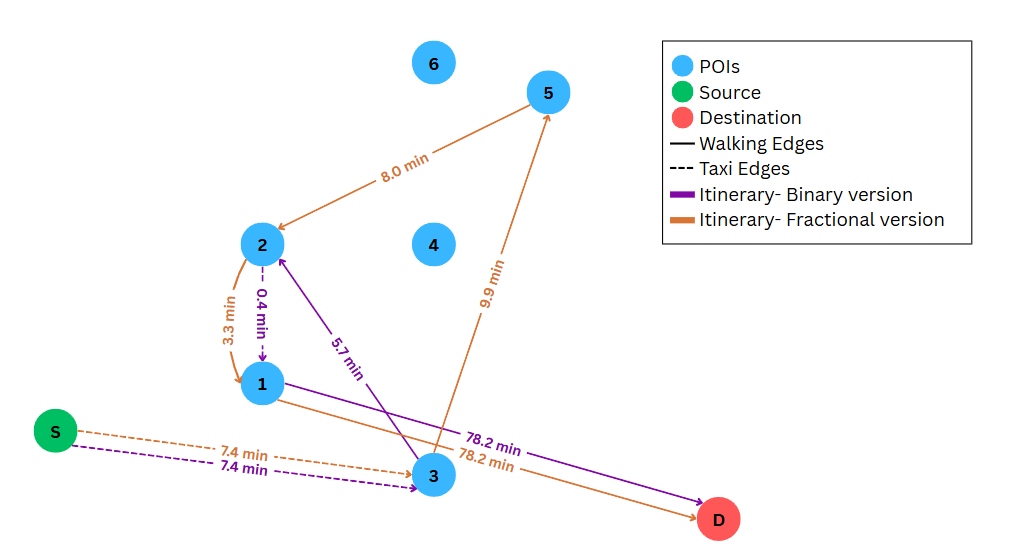
\includegraphics[width=0.5\textwidth]{toy.png}
\caption{Toy Example}
\label{fig:sample_image}
\end{figure}

\noindent \textbf{Itinerary suggested in Binary Version:}
Start from S, spend exact amount of visiting time on POIs 1,2 and 3 and gain complete utility from them, reach D.
\begin{itemize}
    \item \textbf{Utility Score:} 1738
    \item \textbf{Total trip cost:} 3211 Rupees
    \item \textbf{Total time taken:} 256.75 minutes
\end{itemize}

\noindent \textbf{Itinerary suggested in Fractional Version}\\
\textbf{Variant of utility calculation: Continuous Linear Function}
Start from S, arrive on 3, visit it completely and gain full utility, arrive on 5, visit it completely and gain full utility, arrive on 2, spend 28.14 minutes here instead of 30 minutes, gain proportional utility, then arrive on 1, spend complete visiting time and gain full utility, then reach destination.
\begin{itemize}
    \item \textbf{Utility Score:} 2037.31
    \item \textbf{Total trip cost:} 3475.25 Rupees
    \item \textbf{Total time taken:} 300 minutes
\end{itemize}

\noindent \textbf{Variant of utility calculation: Slabs}
Same itinerary as CLF variant except on POI 2, the utility granted to tourist was $28.14/30$
which is $0.938$ times the complete utility i.e. $237.314$, Here in slabs variant, spending $93.8\%$ utility grants $90\%$ of complete utility according to Slab 5, and tourist will gain the same utility on POI 2 if he spends $27$ minutes here, hence utility granted is $227.7$ and time spent is $27$ minutes instead of $28.14$ minutes.
\begin{itemize}
    \item \textbf{Utility Score:} 2027.7
    \item \textbf{Total trip cost:} 3475.25 Rupees
    \item \textbf{Total time taken:} 298.86 minutes
\end{itemize}

\noindent \textbf{Insights}
\begin{itemize}
    \item Fractional Version gains ~$17\%$ more utility than Binary Version.
    \item More effecient Time and Cost budget utilization can be observed in the Fractional version.
    \item The Slabs variant gives approximately similar utility as CLF variant with slight changes due to the modelling of slabs.
\end{itemize}

\section{ILP Modelling}
\begin{align}
    & \textbf{maximize} \sum_{d \in \text{days}} \sum_{i = 1}^{N} U(v_i) \cdot y_{i,d} \hspace{3.4cm} \ref{eq:multi_day_binary} \notag\\
    & \textbf{subject to:} \notag \\ 
    & \sum_{d \in \text{Days}} y_{i,d} \leq 1 \quad \forall i \in \text{poi\_ids} \setminus \{\mathit{hotel\_id}\}\\
    & \text{day\_visit}_i = \sum_{d \in \text{Days}} d \cdot y_{i,d}\quad \forall i \in \text{poi\_ids} \\
    & z_{i,j,d} = w_{i,j,d} + x_{i,j,d} \quad\forall i, j \in \text{poi\_ids},\, i \ne j,\; \forall d \in \text{days} \\
    & z_{i,j,d} \leq 1 \quad \forall i, j \in \text{poi\_ids},\, i \ne j,\; \forall d \in \text{days} \\
    &  z_{i,j,d} \leq y_{i,d} \quad \forall d \in \text{days},\quad \forall i, j \in \text{poi\_ids},\; i \ne j\  \\
    &  z_{i,j,d} \leq y_{j,d}, \quad \forall d \in \text{days},\quad \forall i, j \in \text{poi\_ids},\; i \ne j\ \\   
    & s_{i,d} \leq day\_start\_time + day\_budget + (1 - y_{i,d}) \cdot M \notag\\
    &\forall i \in \text{poi\_ids}, \forall d \in \text{days}\  \\
    & \textbf{1. First Day } (d = d_1): \notag \\
    & \sum_{\substack{j \in \text{POIs} \\ j \neq \text{starting-poi}}} z_{\text{source-poi},j,d_1} = 1 \\
    & \sum_{\substack{i \in \text{POIs} \\ i \neq \text{hotel}}} z_{i,\text{hotel},d_1} = 1  \\
    & \sum_{\substack{j \in \text{POIs} \\ j \neq \text{hotel}}} z_{\text{hotel},j,d_1} = 0  \\
    & \textbf{2. Last Day } (d = d_T): \notag \\
    & \sum_{\substack{j \in \text{POIs} \\ j \neq \text{hotel}}} z_{\text{hotel},j,d_T} = 1 \\
    & \sum_{\substack{i \in \text{POIs} \\ i \neq \text{ending-poi}}} z_{i,\text{ending-poi},d_T} = 1 \\
    & \sum_{\substack{j \in \text{POIs} \\ j \neq \text{ending-poi}}} z_{\text{ending-poi},j,d_T} = 0 \\
    & \textbf{3. Intermediate Days } (d \in \text{Days} \setminus \{d_1, d_T\}): \notag \\[0.2cm]
    & \sum_{\substack{j \in \text{POIs} \\ j \neq \text{hotel}}} z_{\text{hotel},j,d} = 1 \quad \forall d \in \text{Days} \setminus \{d_1, d_T\} \\
    & \sum_{\substack{i \in \text{POIs} \\ i \neq \text{hotel}}} z_{i,\text{hotel},d} = 1 \quad \forall d \in \text{Days} \setminus \{d_1, d_T\} \\
    & \sum_{\substack{i \in \text{POIs} \\ i \neq k}} z_{i,k,d} = y_{k,d}
    \quad \forall d \in \text{Days},\forall k \in \text{POIs} \setminus \{\text{start}, \text{end}, \text{hotel}\}\\
    & \sum_{\substack{j \in \text{POIs} \\ j \neq k}} z_{k,j,d} = y_{k,d}, \quad \forall d \in \text{Days}, \forall k \in \text{POIs} \setminus \{\text{start}, \text{end}, \text{hotel}\}
     \end{align}
\begin{align}
    & \sum_{i \ne j} t^{w}_{i,j} \cdot w_{i,j,d} + \sum_{i \ne j} t^{t}_{i,j} \cdot x_{i,j,d} + \sum_{i \in V} \text{t}(v_i) \cdot y_{i,d} \nonumber \leq H \hspace{0.9cm} \ref{mul_day_9}\\
    & \sum_{d \in \text{Days}} \sum_{(i,j) \in I} c^{w}_{i,j} \cdot w_{i,j} + c^{t}_{i,j} \cdot x_{i,j} + \sum_{d \in \text{Days}} \sum_{i \in I} c(v_i) \leq B \hspace{0.3cm} \ref{mul_day_25} \notag\\
    & s_{i,d} \geq \left( s_{j,d} + t(v_j) + t^{w}_{j,i,d} \cdot w_{j,i,d} + t^{x}_{j,i,d} \cdot x_{j,i,d} \right) \cdot z_{j,i,d} \notag\\
    &- M_{ji} \cdot (1 - z_{j,i,d}) \quad\forall i \neq j,\; \forall d \in \text{Days} \\
    & ot(v_i) \leq s_{i,d} \leq ct(v_i) - t(v_i) \quad \forall v_i \in V, \forall d \in \text{Days} \hspace{1cm}\ref{mul_day_30} \notag\\
    & y_{i,d} = 0 \quad \forall i \in \text{POIs}, \forall d \in \text{Days} \notag \\& \text{ if } \texttt{day\_availability}[trip\_weekdays][d]][i] = 0 \hspace{1cm}\ref{mul_day_31} \notag\\
    & s_{start\_node,d} = \text{day\_start\_time} \quad \forall d \in \text{days}
\end{align}

The objective function (1) maximises the overall utility of the trip. Constraint (7) ensures that each POI is visited atmost once in the whole trip. Constraint (8) assigns a day to each POI on which it is visited during the itinerary. Constraints (9) and (10) ensure that only one mode out of Taxi and Walk is selected. Constraints (11) and (12) establish a logical connection between edges and vertices by preventing isolated edges and vertices. Constraint (13) puts an upper bound on the arrival time of each POI. Constraints (14),(15) and (16) make sure that the itinerary of first day is correctly modelled from source POI to hotel POI. Similarly, Constraints (17),(18) and (19) make sure that the itinerary of last day is correctly modelled from hotel POI to destination POI, and Constraints (20) and (21) help in modelling the itinerary of intermediate days from hotel to hotel correctly. Constraints (22) and (23) are connectivity constraints, which impose a restriction that if an edge enters a vertex, another edge must leave that vertex. Constraints (2),(3),(5),(6) are time budget, cost budget, opening closing time and opening closing day constraints respectively that are already explained in previous section. Constraint (24) ensures that if an edge goes from POI j to POI i, then the arrival time of i is greater than or equal to the sum of visit time of POI j and travel time between j to i. M is a large constant which relaxes the constraint when both of them aren't part of itinerary. Constraint (25) ensures that each day's itinerary starts on correct time as stated by the tourist.

\section{Personalized Constraints}
\begin{itemize}
\item \textbf{Must-see POIs}\\
This constraint enforces that each POI marked as a must-see is visited exactly once over the duration of the trip:

\begin{equation}
\label{mul_day_7}
    \sum_{d \in \text{days}} y_{i,d} = 1 \quad \quad \forall i \in \text{must\_see\_pois}
\end{equation}

where:
\begin{itemize}
  \item \texttt{must\_see\_pois} is the set of user-specified must-visit POIs
\end{itemize}
\item \textbf{Must-avoid POIs}\\
This constraint enforces that each POI marked as excluded is never visited in the entire trip:

\begin{equation}
\label{mul_day_8}
    \sum_{d \in \text{days}} y_{i,d} = 0 \quad \quad \forall i \in \text{excluded\_pois}
\end{equation}

where:
\begin{itemize}
  \item \texttt{excluded\_pois} is the set of user-specified excluded POIs
\end{itemize}
\item \textbf{Category Constraints}\\
The user can specify the lower bound and upper bound for the categories of POIs to be visited across the trip. This constraint ensures that user's preferences over these themes are respected:

\begin{align}
\label{mul_day_11}
lb_m \leq \sum_{i \in V_m} \sum_{d \in \text{days}} y_{i,d} \leq ub_m, \quad \forall m \in C 
\end{align}

where:
\begin{itemize}
  \item \( C \) represents all the categories (e.g., historical, cultural, adventure, etc.)
  \item \( lb_m \) and \( ub_m \) are the lower and upper bounds for theme \( m \)
\end{itemize}
\item \textbf{Ordering Constraints}\\
If (a,b) is an ordering constraint, then POI a and POI b can be visited on different days, so this constraint makes sure that day of visit of POI a is before, or same as day of visit of POI b.
\begin{align}
\label{mul_day_12}
\texttt{day\_visit}_a \leq \texttt{day\_visit}_b, \quad \forall (v_a, v_b) \in P
\end{align}
\noindent
where:
\begin{itemize}
    \item \( \texttt{day\_visit}_a \): the day on which POI \( a \) is visited.
    \item \( P \): the set of all ordered POI pairs with ordering constraints entered by the tourist.
\end{itemize}

\textbf{2. Intra-day Temporal Ordering Constraint}\\
If (a,b) is an ordering constraint and both POI a and POI b are to be visited on same day, then this constraint ensures that arrival time of POI b is greater than or equal to sum of arrival time of POI a, visit duration of POI a and travel time from POI a to POI b.

\begin{align}
\label{mul_day_13}
s_{i,d} + \left( t(v_i) + \left( t^{w}_{i,j} \cdot w_{i,j,d} + t^{t}_{i,j} \cdot x_{i,j,d} \right) \right) y_{i,d}
&\leq s_{j,d} + T_{ij} (1 - y_{j,d})\\ \forall (v_i, v_j) \in P,\; \forall d \in \text{days} \nonumber \\
\label{mul_day_14}
T_{ij} = ct(v_i) + t(v_i) + t^{w}_{i,j} 
\end{align}



\noindent
where:
\begin{itemize}
    \item \( s_{i,d} \): start time of visiting POI \( i \) on day \( d \).
    \item \( t(v_i) \):visit time spent at POI \( i \).
    \item \( ct(v_i) \): closing time of POI \(v_i\) \( i \).
\end{itemize}

\noindent
The Big-M term \( T_{ij} (1 - y_{j,d}) \) ensures the constraint becomes non-restrictive when POI \( j \) is not selected on day \( d \).
\end{itemize}

\section{Major Contributions}
\textbf{Dynamic Re-routing}\\
The real tourist behavior and weather conditions, are dynamic and unpredictable in nature. They can be influenced by unforeseen delays, detours, longer-than-anticipated visits, or spontaneous user preferences, which can significantly impact the feasibility and correctness of an advanced preplanned itinerary. To close the gap between theory and practice, a dynamic approach is required.

In contrast with the static approach used in \cite{taylor2018tour}, where rigid, precomputed travel times and POI visit times, we have taken real-time travel times using Google-Maps API (Routes API). 

On the top of suggested times of visit and travel, user can enter the actual time they have taken to visit a POI and the travel time they took to reach the current POI.

With every visit to a POI, the system replans the schedule based on the remaining time and cost budgets. The POIs already visited are not considered for further itineraries. This optimizes the rest of the day based on current progress and not stale assumptions.

For the dynamic feature, a record of visited POIs was maintained. On visiting a POI, it was eliminated from the list to be taken into account in future itinerary calculations with the new remaining time and cost budgets.

\begin{figure}[H]
\textbf{Implementation of Dynamic Approach}
\centering
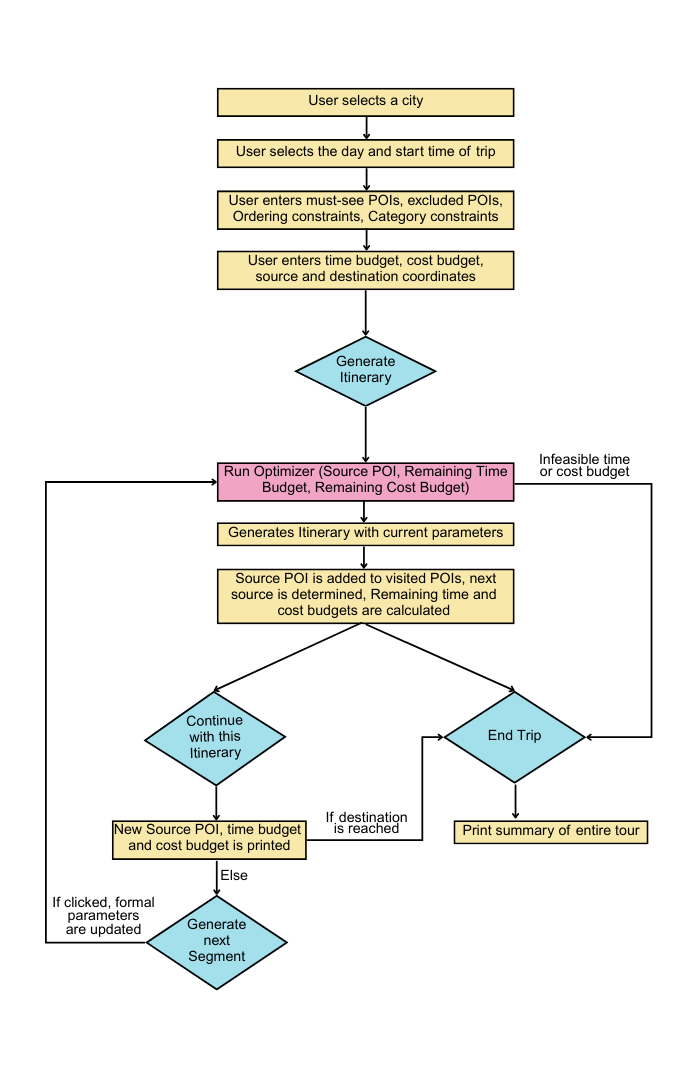
\includegraphics[width=0.5\textwidth]{binary dynamic flowchart.png}
\caption{Implementation of Dynamic Approach}
\label{fig:flowchart_dynamic}
\end{figure}

\noindent \textbf{Fractional Visits to POIs}\\
This feature enables partial visiting of Points of Interest (POIs), thus enhancing the flexibility and potential utility of the proposed itineraries. In comparison to the Binary approach used before which required the POI to be completely visited in order to collect its utility, the Fractional version built here grants proportional utility based on the proportion visited of the POI—improving time and cost budget efficiency.

\textbf{Fractional POI Variable (ppoi[i])}
\begin{itemize}
    \item A real variable $\text{ppoi}[i] \in [0, 1]$ is defined for every POI i to reflect the portion of the POI's total visit time covered by the itinerary.

    \item A threshold of 0.5 (50\%) is enforced: POIs must be visited for at least half of their average duration to be included. If ppoi[i] < 0.5, it is effectively set to 0 and the POI is excluded from the plan.
\end{itemize}

\textbf{Utility Calculation Variants}
\label{Utility_Calculation}

Two distinct methods are used to compute the utility in the fractional setting:

\begin{itemize}
\item {Continuous Linear Utility Model}

In this version, the utility granted is directly proportional to the fraction of the POI visited.

If a POI has utility $U$ and is visited for $p$ fraction of time (where $p \in [0.5, 1]$), the utility granted is $U \times p$.

\item{Slab-Based Utility Model}
\begin{itemize}[noitemsep, topsep=0pt]
    \item Fraction $\in$ [0.5, 0.6) $\rightarrow$ 50\% utility
    \item Fraction $\in$ [0.6, 0.7) $\rightarrow$ 60\% utility
    \item Fraction $\in$ [0.7, 0.8) $\rightarrow$ 70\% utility
    \item Fraction $\in$ [0.8, 0.9) $\rightarrow$ 80\% utility
    \item Fraction $\in$ [0.9, 1.0) $\rightarrow$ 90\% utility
    \item Fraction = 1.0 $\rightarrow$ 100\% utility
\end{itemize}

It is important to note that we provide 100\% utility if and only if POI is visited completely. The utility granted coincides with the lower bound because we do not want a situation like this to occur where even if we suggest that tourist visit 50\% POI and they get any utility greater than 50\% because that would scale up the actual utility as compared to the continuous linear function.
\end{itemize}

To enable fractional visits, the constraints were modified to make the visit duration at one POI proportional to a continuous variable \( ppoi_i \in [0,1] \), that represents the relative fraction of the overall visit duration spent at the POI \( v_i \). Accordingly, in all the constraints, the original visit times are multiplied by this fractional variable \( ppoi_i \), ensuring the constraints accurately reflect partial visits.

When the utility function is a continuous linear function of visit time, the utility score obtained from a POI is also scaled proportionally, i.e., \( \text{utility}_i = U(v_i) \cdot ppoi_i \), where \( U(v_i) \) is the full utility for a complete visit to POI \( v_i \).

For the slab-based utility variant, a continuous variable \( \text{effective\_utility}_i \) is used to capture the actual utility awarded based on the fraction of time spent at each POI. The utility is determined using discrete slab multipliers based on the visit duration. Each POI is assigned to at most one slab, and the utility is calculated as:

\begin{align}
\label{effective_utility}
\text{effective\_utility}_i &= U(v_i) \cdot \big(0.5 \cdot s_1[i] + 0.6 \cdot s_2[i] + 0.7 \cdot s_3[i] \notag \\
&\quad + 0.8 \cdot s_4[i] + 0.9 \cdot s_5[i] + 1.0 \cdot s_6[i] \big)
\end{align}

The optimization objective is to maximize the total utility accumulated across all POIs:

\begin{align}
\label{objective_fun_slabs}
U(I) = \sum_{i=1}^N \text{effective\_utility}_i
\end{align}

To ensure only one slab level is chosen per POI, the following constraint is imposed:

\begin{align}
\sum_{k=1}^{6} s_k[i] \leq 1, \quad \forall i \in \{1, \dots, N\}
\end{align}


\section{Experiments}
\subsection{Dataset Description}
In order to test our itinerary planning system, we used curated sets of Points of Interest (POIs) for seven large cities namely: Delhi, Budapest, Vienna, Osaka, Glasgow, Edinburgh, and Perth. The initial dataset utilized is derived from the \textbf{Yahoo Flickr Creative Commons 100 Million Dataset (YFCC100M)}, containing near about 100 million images, of which 69 million are annotated and 48 million are geotagged.

We used the Flickr User-POI Visits dataset available at ~\cite{limkwanhuiDataCode}, which was generated in a below explained manner; In order to generate this dataset the authors of the paper ~\cite{taylor2018tour} took a set of popular POIs for every city mentioned earlier using resources such as \textit{Wikipedia}. Then, geotagged photos in \textit{Flickr} were matched with these POIs using spatial proximity. By estimating relative \textbf{popularity} of a POI through the counts of photos for every POI, the relative popularity which is referred to as utility was estimated.

This approach generates an empirical proxy for real tourist behavior, measuring interest in a specific attraction as measured by publicly accessible, crowd-sourced images.

The existing dataset contained the following key fields for each POI:

\begin{table}[H]
\begin{tabularx}{0.5\textwidth}{p{3cm} X}
\hline
\textbf{Field Name} & \textbf{Description} \\
\hline
\texttt{poiID} & A unique identifier assigned to each POI. \\
\hline
\texttt{poiName} & The name of the POI, e.g., ``Red Fort'', ``Osaka Castle''. \\
\hline
\texttt{lat} & Latitude coordinate of the POI. \\
\hline
\texttt{long} & Longitude coordinate of the POI. \\
\hline
\texttt{theme or category} & Thematic classification of the POI, such as \textit{amusement}, \textit{historical}, \textit{museum}, \textit{shopping}, \textit{park}, etc. \\
\hline
\texttt{Utility Score or Profit} & A numerical value representing the estimated utility or attractiveness of the POI, derived based on its popularity (photo frequency). \\
\hline
\texttt{Cost} & Geospatial travel distance (in meters) between pairs of POIs. This is used in the travel time estimation between locations considering the walking speed to be 4 kmph and taxi speed as 30kmph which can be modified as per requirement. \\
\hline
\end{tabularx}
\caption{Original dataset fields}
\end{table}

With an aim to make our system more authentic and feasible to use, we supplemented the dataset manually with real-life operating limitations and data that we gathered from \textbf{official tourist websites} and verified online portals. The added fields are:

\begin{table}[H]
\centering
\begin{tabularx}{0.5\textwidth}{p{3cm} X}
\toprule
\textbf{Field Name} & \textbf{Description} \\
\midrule
\texttt{fees} & Entrance fee or ticket price associated with the POI, in INR. \\
\midrule
\texttt{opening time} & The time at which the POI opens for visitors, stored in \texttt{HH:MM:SS} format. \\
\midrule
\texttt{closing time} & The time at which the POI closes for visitors, stored similarly. \\
\midrule
\texttt{Days of Week} & Seven binary columns (\texttt{Monday}, \texttt{Tuesday}, ..., \texttt{Sunday}). A value of 1 indicates the POI is open on that day; 0 indicates it is closed. \\
\midrule
\texttt{Avg Visiting Time} & The average duration (in minutes) tourists typically spend at the POI. \\
\bottomrule
\end{tabularx}
\caption{Additional features added to the dataset}
\end{table}



These manually extracted features add a \textbf{temporal and availability aspect} to the optimisation problem, allowing more realistic and accurate itinerary generation. For example, POIs closed on the chosen day are excluded from the planning automatically.

All the other information was collected by scraping or quoting \textbf{official tourist boards}, \textbf{city tourism websites}, and trustworthy travel websites.

The experiments were conducted on a MacBook Air equipped with an Apple M1 processor and 8GB of RAM, providing a lightweight yet efficient environment for developing and testing the itinerary planning system. The implementation was carried out in Python, leveraging its rich ecosystem for data handling, user interaction, and visualization. The core optimization process was performed using the Gurobi Optimizer, a state-of-the-art solver for mathematical programming. Gurobi was employed to solve the underlying Integer Linear Programming (ILP) formulations that generate optimized multi-day travel itineraries under various user-defined constraints and real-world conditions.

\subsection{Baseline Itinerary Planner}

To establish a baseline for evaluation, we implemented the itinerary planning model described in the widely cited WWW paper, which we refer to as the \textbf{baseline model}. This model adopts a binary decision framework where each Point of Interest (POI) is either fully included in the itinerary or completely excluded. The utility function in this setting is defined as:

\[
\max \left\{ \sum_{i=2}^{N} \sum_{j=2}^{N} S_i \cdot x_{i,j} \right\}
\]

where \( x_{i,j} = 1 \) if POI \( i \) is visited immediately before POI \( j \), and 0 otherwise. This is equivalent to the binary utility formulation:

\[
\sum_{i=1}^{N} U(v_i) \cdot y_i
\]

where \( U(v_i) \) denotes the utility of POI \( v_i \), and \( y_i \in \{0,1\} \) is a binary variable indicating whether \( v_i \) is selected in the itinerary.

The baseline model incorporates only fundamental constraints, including the time budget constraint, connectivity requirements, a restriction preventing a direct path between the start and end POIs, and a sub-tour elimination constraint. In our implementation, the sub-tour elimination is effectively enforced using arrival-time-based constraints. We were able to seamlessly adapt our ILP-based framework to replicate this baseline behavior, effectively converting our advanced planner into a simplified version matching the baseline model's structure.

However, direct performance comparison between our model and the baseline was not feasible due to a key limitation in the common dataset used by both our system and the WWW paper---namely, the absence of standardized POI visiting durations. Second, the baseline paper distributed POI visit durations by an unspecified method, making it impossible to reproduce exactly the same execution cases. Despite this, we were able to re-implement the baseline model in its entirety in terms of constraints as well as utility structure, which provided a good basis for qualitative analysis.

\subsection{Input and Performance Metrics}

Directly from thesis

\subsection{Demonstrations}

\subsection{Conclusion}

% PREVIOUS CONTENT COMMENT BEGINS

% Each POI \( v_i \in V \) has the following attributes:

% \begin{itemize}
%     \item \( [ot(v_i), ct(v_i)] \): Opening time and closing time of the POI.
%     \item \( U(v_i) \): Weight denoting the importance of the POI (utility score).
%     \item \( t(v_i) \): Average time tourists spend at the POI.
%     \item \( c(v_i) \): Entrance fee for the POI.
% \end{itemize}

% \textbf{Multimodal Graph Representation:}
% This problem is represented as a multimodal graph \( G = (V, E) \) where:

% \begin{itemize}
%     \item \( V = \{v_1, ..., v_N\} \) represents the set of POIs.
%     \item \( E \) consists of two edges between each pair of POIs \( (v_i, v_j) \):
%     \begin{itemize}
%         \item \textbf{Walking Edge} \( e^{w}_{i,j} \) with attributes:
%         \begin{itemize}
%             \item \( t^{w}_{i,j} \): Time required to walk from \( v_i \) to \( v_j \).
%             \item \( c^{w}_{i,j} \): Cost associated with walking (typically zero).
%         \end{itemize}
%         \item \textbf{Taxi Edge} \( e^{t}_{i,j} \) with attributes:
%         \begin{itemize}
%             \item \( t^{t}_{i,j} \): Time required to travel by taxi.
%             \item \( c^{t}_{i,j} \): Cost of travel by taxi.
%         \end{itemize}
%     \end{itemize}
% \end{itemize}

% % This problem can be represented as a graph \( G = \langle V , E \rangle \) where \( N = |V| \), \( V = \{v_1, ..., v_N\} \) represents the set of vertices (POIs), and \( E \) is the set of connecting edges. Each edge \( e_{i,j} \) connecting vertex \( i \) to \( j \) has a travel time cost \( t_{i,j} \) and a travel cost \( c_{i,j} \).

% \section{Objective}

% The objective is to generate a single-day itinerary $I$ which is an ordered subset of \( V \) that maximizes the total utility score while maintaining budget and time constraints. The itinerary $I$ is a sequence of POIs selected from the given set \( V \), ensuring that the tourist can visit these locations feasibly within the available time and budget.

% \subsection{Utility Score Maximization}

% Each POI \( v_i \in V \) has an associated utility score \( U(v_i) \) that represents its desirability or importance to the tourist.

% The total utility score of an itinerary \( I \) is given by:

% \begin{align}
% U(I) &= \sum_{v_i \in I} U(v_i) \notag
% \end{align}

% Let $y_i$ is a binary variable that takes value $1$ if the itinrary visits the POI $v_i$; and  $0$ otherwise. Then, the above constraint can be written as:
% \begin{align}
% U(I) &= \sum_{i=1}^N U(v_i) \times y_i \label{1}
% \end{align}
% The goal is to determine an itinerary $I$ with maximum utility $U(I)$, such that the following constraints are satisfied.

% \section{Constraints}

% \subsection{Starting and Ending point Constraint}
% \noindent
% This constraint ensures that exactly one outgoing edge is selected from the starting node $v_1$ and no incoming edge is selected for the starting node. Similarly, for the ending node of the itinerary, $v_N$, exactly one incoming edge must be selected and no outgoing edge must be selected in the itinerary. 
% Mathematically, this is expressed as follows:
% \begin{align}
% \sum_{j=2}^{N} z_{1,j} &= 1 \label{2} \\  
% \sum_{i=2}^N z_{i,1} &= 0 \label{3} \\
% \sum_{i=1}^{N-1} z_{i,N} &= 1 \label{4} \\
% \sum_{j=1}^{N-1} z_{N,j} &= 0 \label{5}
% \end{align}


% Where $z_{i,j}$ is a binary variable that takes value $1$ if the path from node $v_i$ to $v_j$ is selected in the itinerary; and $0$ otherwise. Here $1$ and $N$ denote the starting node and the ending node of the itinerary. For simplicity, it is also assumed that the total number of POIs is $N$. 

% \subsection{No Self Loops}
% This constraint ensures that there is no edge from any vertex to itself.

% \begin{align}
% z[i, i] = 0 \quad \forall i \in V \label{6}
% \end{align}


% \subsection{Connectivity Constraint:}

% \noindent
% This constraint ensures that:
% \begin{itemize}
%     \item Each Point of Interest (POI) can be \textbf{visited at most once}, preventing cycles or repeated visits to the same node.
%     \item All selected nodes are \textbf{connected in a single continuous path}.
% \end{itemize}

% In other words, if an intermediate POI, $v_I \in V\setminus \{v_1,v_N\}$ is visited, then there must be exactly one incoming edge and exactly one outgoing edge 
% from the given POI, must be selected in the itinerary.
% \begin{align}
% \sum_{i=1}^{N-1} z_{i,k} = \sum_{j=2}^{N} z_{k,j} = y[k] &\le 1, \label{7}
% \end{align}


% \subsection{Logical Connection Between variables $y$ and $z$}
% \noindent
% This constraint ensures that $z_{i,j}=1$ if and only if both $y_i=1$ and $y_j=1$. Mathematically, this can be represented as:
% \begin{align}
% z_{i,j} &\leq y_i  &\forall i, j \in \{ 1, \dots, N \}, \ i \neq j \label{8} \\
% z_{i,j} &\leq y_j &\forall i, j \in \{ 1, \dots, N \}, \ i \neq j \label{9} \\
% y_i &\le \sum_{j=1}^N z_{i,j} &\forall i=\{1,\dots,N-1\}, \ i \neq j \label{10}\\  
% y_j &\le \sum_{i=1}^N z_{i,j} &\forall j=\{2,\dots,N\}, \ i \neq j \label{11} 
% \end{align}


% \subsection{Subtour Elimination Constraint}

% This constraint ensures that subtours (loops that do not include the starting or ending POIs) are eliminated, maintaining a continuous and feasible route throughout the itinerary.

% \begin{align}
% 2 \leq p_i \leq N, &&\forall i = 2, \ldots, N &\label{12} \\
% p_i - p_j + 1 \leq (N - 1)(1 - z_{i,j}),  &&\forall i, j = 2, \ldots, N &\label{13}
% \end{align}

% where $p_i$ represents the position of POI \( v_i \) in the itinerary sequence.
     

% Equation (1) ensures that the position values are within the valid range, while Equation (2) prevents the formation of subtours by enforcing logical sequencing constraints between POIs.

% \subsection{Mode Selection Constraint}
% This constraint ensures that for every pair of POIs, the tourist can choose only one mode of transportation, either walking or taking a taxi.

% \begin{align}
%     w_{i,j} + x_{i,j} &= z_{i,j} \leq 1&\forall edge (v_i, v_j) \in E \label{14}
% \end{align}

% \text{Where:}

% \begin{align}
% w_{i,j} &= 
% \begin{cases} 
% 1 & \text{if walking is chosen between nodes } i \text{ and } j \\ 
% 0 & \text{otherwise} 
% \end{cases} \label{15}\\[8pt]
% x_{i,j} &= 
% \begin{cases} 
% 1 & \text{if taxi is chosen between nodes } i \text{ and } j \\ 
% 0 & \text{otherwise} 
% \end{cases} \label{16}
% \end{align}




% \subsection{Maximum Walking Time Constraint}
% \begin{itemize}
% \item This constraint limits the maximum continuous walking duration between any two POIs to ensure the tourist does not walk excessively long without rest.

% \[
%     t^{w}_{i,j} \cdot w_{i,j} \leq X \quad \forall (v_i, v_j)\in I
% \]

% Where \( X \) is the maximum continuous walking duration (45 minutes).
% \end{itemize}

% \subsection{Time Constraint}
% \begin{itemize}
%     \item The total time spent in the itinerary, including both visit time and travel time, must not exceed the available time \( H \):

%     \begin{align}
%          \sum_{(i,j) \in I} (t^{w}_{i,j} \cdot w_{i,j} + t^{t}_{i,j} \cdot x_{i,j}) + \sum_{i \in I} t(v_i) \leq H \label{17}   
%     \end{align}
 
%     Here, \( H \) is the maximum allowable time (e.g., a single day's duration) for completing the trip.
% \end{itemize}

% \subsection{Budget Constraint}
% \begin{itemize}
%     \item The total cost of the itinerary \( I \), including both POI costs and travel costs, must not exceed the available budget \( B \):

%     \begin{align}
%     \sum_{(i,j) \in I} (c^{w}_{i,j} \cdot w_{i,j} + c^{t}_{i,j} \cdot x_{i,j}) + \sum_{i \in I} c(v_i) \leq B \label{18}
%     \end{align}

%     \item Here, \( B \) is the maximum allowable budget for the trip.
% \end{itemize}

% \subsection{Ordering Constraint}
% \begin{itemize}
%     \item Certain POIs must be visited before others due to dependencies, operational constraints, or logical sequencing (e.g., visiting a particular temple before another temple).
%     \item Let \( P \subseteq V \times V \) be the set of ordered POI pairs \( (v_i, v_j) \), where POI \( v_i \) must be visited before POI \( v_j \).
%     \item Let \( s_i \) and \( s_j \) denote the times when the tourist reaches the POIs \( v_i \) and \( v_j \), respectively.
%     \item Each POI \( v_i \) has a visit duration \( t(v_i) \), and traveling from \( v_i \) to \( v_j \) takes \( t_{i,j} \).
%     \item Let \( y_i \) be a binary variable where \( y_i = 1 \) if POI \( v_i \) is included in the itinerary, and \( y_i = 0 \) otherwise.
%     \item \( T_{ij} \) is a sufficiently large constant to deactivate the constraint when \( v_j \) is not selected.
    
%     \begin{align}
%     s_i + (t(v_i) + t_{i,j}) y_i &\leq s_j + T_{ij} (1 - y_j), \quad \forall (v_i , v_j) \in P \label{19} \\
%     T_{ij} &= ct(v_i) + t(v_i) + t_{ij} \label{20}
%     \end{align}

% \end{itemize}

% \subsection{Category Constraint}
% \begin{itemize}
%     \item The number of POIs selected from each category is bounded by predefined lower and upper limits.
%     \item Let \( C \) denote the set of all categories.
%     \item For each category \( m \in C \), let \( V_m \subseteq V \) represent the set of POIs belonging to that category.
%     \item Let \( y_i \) be a binary variable where \( y_i = 1 \) if POI \( v_i \) is included in the itinerary, and \( y_i = 0 \) otherwise.
%     \item Let \( lb_m \) and \( ub_m \) denote the lower and upper bounds, respectively, on the number of POIs to be selected from category \( m \).

%     \begin{align}
%     lb_m \leq \sum_{i \in V_m} y_i \leq ub_m, \quad \forall m \in C \label{21}
%     \end{align}

%     \item The value of \( lb_k \) for any mandatory category \(k \in m\) will be 1.
% \end{itemize}

% % \subsection{Opening and Closing time Constraint}
% % \noindent
% % This constraint ensures that the tourist arrives at the POI between its opening and closing time and has enough time to explore that POI properly. \\

% % Mathematically, this is expressed as:
% % \begin{align}
% % ot(v_i) \leq s_i \leq ct(v_i) - t(v_i) \quad \forall v_i \in V \label{22}
% % \end{align}

% \subsection{Opening and Closing Time Constraint}
% \noindent
% This constraint ensures that the tourist arrives at the POI between its opening and closing time and has enough time to explore that POI properly. \\

% Mathematically, this is expressed as:
% \begin{align}
% ot(v_i) \leq s_i \leq ct(v_i) - t(v_i) \quad \forall v_i \in V \label{22}
% \end{align}

% Additionally, this constraint also plays a crucial role in preventing the formation of sub-tours. Specifically, if a sub-tour were to form, the arrival time constraint  
% \begin{align}
% arrival\_time[j] \geq arrival\_time[i] + travel\_time(i, j)
% \end{align}
% would fail when applied between the last node and the starting node of the loop, as the time constraints would not be satisfied. This ensures that no disconnected cycles can exist in the itinerary, maintaining a valid and continuous tour.\\

% Along with this there is an additional constraint that arrival time at any poi should be upper bounded by sum of trip starting time and given time budget.
% \[a_i \leq t_s + T,\]
% \text{where } $a_i$ \text{ is arrival time at POI } $i$,\ $t_s$ \text{ is trip start time, and } $T$ \text{ is time budget.}





% \subsection{Opening and Closing Day constraint}
% \noindent
% This constraint ensures that the tourist arrives at the POI on the day when it is open.\\[0.2cm]
% 1. $d_{i,k}$ is a binary variable for each POI and day of the week:
% \begin{align}
% d_{i,k} =
% \begin{cases}
%     1 & \text{if POI } i \text{ is open on day } k \\[0.2cm]
%     0 & \text{otherwise}
% \end{cases} \label{23}
% \end{align}

% \noindent 2. \textbf{Constraint for availability:}
% Let $Weekday = \{Monday, \ldots, Sunday\}$.
% \begin{align}
%     y_i \cdot d_{i,k} = y_i \quad \quad \forall i \in V, \forall k \in Weekday \label{24}
% \end{align}



% \section{Integer Linear Program for the Itinerary Planning Problem (ILP-IPP)}

% \begin{align}
%     & \textbf{maximize} \sum_{v_i \in V} U(v_j)\times y_i \notag &\ref{1} \\
%     & \textbf{subject to:} \notag \\ 
%     & \sum_{j=2}^{N} z_{1,j} = 1 &\ref{2} \notag\\
%     & \sum_{i=2}^{N} z_{i,1} = 0 &\ref{3} \notag\\
%     & \sum_{i=1}^{N-1} z_{i,N} = 1 &\ref{4} \notag \\
%     & \sum_{j=1}^{N-1} z_{N,j} = 0 &\ref{5} \notag \\
%     & z[i, i] = 0 \quad \forall i \in V &\ref{6} \notag\\
%     &\sum_{i=1}^{N-1} z_{i,k} = \sum_{j=2}^{N} z_{k,j} = y[k] \hspace{4.3cm} \forall k \in \{2, \dots, N-1\} &\ref{7} \notag \\
%     & z_{i,j} \leq y_i \hspace{6.6cm} \quad \forall i, j \in \{ 1, \dots, N \}, \ i \neq j &\ref{8} \notag \\[0.2cm]
%     & z_{i,j} \leq y_j \hspace{6.6cm} \quad \forall i, j \in \{ 1, \dots, N \}, \ i \neq j &\ref{9} \notag \\[0.2cm]\
%     &y_i \le \sum_{j=1}^{N} z_{i,j} \quad \forall i \in \{1,\ldots,N-1\},\, i \neq j &\ref{10} \notag \\[0.2cm]
%     &y_j \le \sum_{i=1}^{N} z_{i,j} \quad \forall j \in \{2,\ldots,N\},\, i \neq j &\ref{11} \notag
%     \end{align}

%     \begin{align}
%     & z_{i,j} = x_{i,j}+w_{i,j} \leq 1 \hspace{5.1cm} \forall (v_i, v_j) \in V &\ref{14} \notag\\[0.2cm]
%     & \sum_{(i,j) \in I} (t^{\text{w}}_{i,j} \cdot w_{i,j} + t^{\text{t}}_{i,j} \cdot x_{i,j}) + \sum_{i \in I} t(v_i) \leq H \hspace{1.5cm} &\ref{17} \notag \\[0.3cm]
%     & \sum_{(i,j) \in I} (c^{\text{w}}_{i,j} \cdot w_{i,j} + c^{\text{t}}_{i,j} \cdot x_{i,j}) + \sum_{i \in I} c(v_i) \leq B \hspace{1.5cm} &\ref{18} \notag\\[0.3cm]
%     & s_i + (t(v_i) + t_{i,j})y_i \leq s_j + T_{ij}(1 - y_j) \hspace{2.5cm} \forall (v_i, v_j) \in P &\ref{19} \notag\\[0.3cm]
%     & T_{ij} = ct(v_i) + t(v_i) + t_{ij} &\ref{20} \notag\\[0.3cm]
%     & l_b^m \leq \sum_{i \in V_m} y_i \leq u_b^m \hspace{5.4cm} \forall m \in C &\ref{21} \notag\\[0.2cm]
%     & ot(v_i) \leq s_i \leq ct(v_i) - t(v_i) \quad \hspace{3.84cm} \forall v_i \in V &\ref{22} \notag\\[0.3cm]
%     & y_i = y_i \cdot d_{i,k} \quad \hspace{6.05cm} \forall i \in V &\ref{24} \notag \\[0.3cm]
%     &d_{ik} \in \{0,1\}  \hspace{6.5cm} \forall i \in \{ 1, \dots, N \}, k \in Weekday &\ref{23} \notag\\ 
%     &x_{ij} \in \{0,1\}  \hspace{6.5cm} \forall i, j \in \{ 1, \dots, N \}, \ i \neq j &\ref{16} \notag\\
%     &y_i \in \{0,1\}  \hspace{6.7cm} \forall i \in \{ 1, \dots, N \} &\ref{15} \notag\\ 
%     &z_{ij} \in \{0,1\}  \hspace{6.55cm} \forall i, j \in \{ 1, \dots, N \}, \ i \neq j &\ref{14} \notag\\
%     &w_{ij} \in \{0,1\}  \hspace{6.5cm} \forall i, j \in \{ 1, \dots, N \}, \ i \neq j &\ref{15} \notag
%     \end{align}

%\subsection{Space-complexity of ILP-IPP}
% \subsection{Size of ILP-IPP}
% There are two factors that contribute to the size of ILP-IPP -- number of variables and number of constraints. We will analyze each of them separately.

% \subsubsection{Number of variables}
% There are five sets of variables: $d, x, y, z, w$. The total number of variables of the type $d$ is $O(N)$, since $|Weekday| = O(1)$ is a constant. The total number of variables of the types $x, y, w$ is $O(N^2)$. The total number of variables of the type $y$ is $O(N)$.

% Hence, the total number of variables in ILP-IPP is $O(N^2)$.

% \subsubsection{Number of constraints}
% A careful analysis of all the constraints shows that the total number of constraints is $O(N^2 + |V| + |P| + |C|)$.\\

% \noindent Combining the two results, we conclude that the size of ILP-IPP is $O(N^2 + |V| + |P| + |C|)$.

% \vspace{3cm}
% \section{Example}

% \begin{figure}[ht] % 'ht' allows placement here or at the top
%     \centering
%     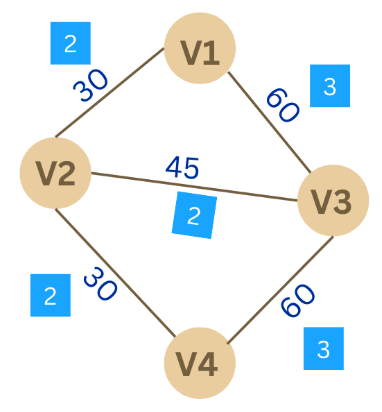
\includegraphics[width=0.3\textwidth]{image1.png} % Adjust width as needed
%     \label{fig:example}
% \end{figure}

% \begin{itemize}
%     \item Time Budget: 6 hours (08:00 - 14:00)
%     \item Cost Budget: 14 units
% \end{itemize}

% \begin{table}[ht]
% \centering
% \begin{tabular}{|c|c|c|c|c|c|}
% \hline
% POI & Opening Time & Closing Time & Utility Score & Visit Time & Entrance Cost \\
% \hline
% \( v_1 \) (Start) & 08:00 & 18:00 & 0 & 0 & 0 \\
% \( v_2 \) & 08:30 & 17:00 & 8 & 1h & 5 \\
% \( v_3 \) & 09:00 & 16:00 & 5 & 1.5h & 3 \\
% \( v_4 \) (End) & 08:00 & 18:00 & 0 & 0 & 0 \\
% \hline
% \end{tabular}
% \caption{POI Details}
% \end{table}

% \subsection{Case 1: \( v_1 \to v_2 \to v_3 \to v_4 \)}
% \begin{itemize}
%     \item \textbf{Travel Cost: } \( 2 + 5 + 2 + 3 + 3 = 15 \) (Invalid, exceeds 14 units)
% \end{itemize}

% \subsection{Case 2: \( v_1 \to v_3 \to v_4 \)}
% \begin{itemize}
%     \item \textbf{Travel Cost:} \( 3 + 3 + 3 = 9 \) (Valid)
%     \item \textbf{Time Taken:}
%     \begin{itemize}
%     \item Travel \( V_1 \to V_3 \) = 09:00
%     \item Visit \( V_3 \) = 10:30
%     \item Travel \( V_3 \to V_4 \) = 11:30 (Valid)
%     \end{itemize}
%     \item \textbf{Utility Score: } 5
% \end{itemize}

% \subsection{Case 3: \( v_1 \to v_2 \to v_4 \)}
% \begin{itemize}
%     \item \textbf{Travel Cost: } \( 2 + 5 + 2 = 9 \) (Valid)
%     \item \textbf{Time Taken:}
%     \begin{itemize}
%     \item Travel \( V_1 \to V_2 \) = 08:30
%     \item Visit \( V_2 \) = 09:30
%     \item Travel \( V_2 \to V_4 \) = 10:00 (Valid)
%     \end{itemize}
%     \item \textbf{Utility Score: } 8 (Best Itinerary)
% \end{itemize}


% \begin{figure}[!]
%     \centering
%     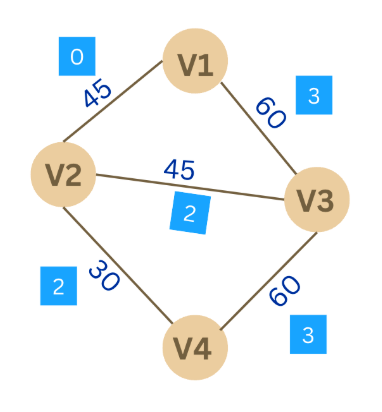
\includegraphics[width=0.3\textwidth]{image2.png} % Adjust width as needed
%     \label{fig:example}
% \end{figure}

% \vspace{5cm}
% \section{Updated Itinerary Consideration}

% Previously, the best itinerary had a utility score of 8. Now, suppose the tourist walks to reach \( V_2 \) from \( V_1 \), which takes 45 minutes, and the cost of transportation reduces to 0. This adjustment changes the best itinerary, resulting in an even higher utility score.\\

% \begin{center}
%     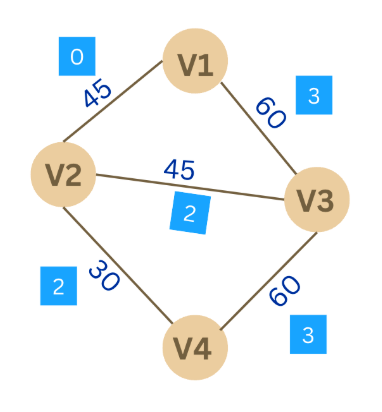
\includegraphics[width=0.3\textwidth]{image2.png}
% \end{center}

% \textbf{Updated Itinerary:}  
% \( V_1 \to V_2 \to V_3 \to V_4 \)\\

% \textbf{Travel Cost:}  
% \( 0 + 5 + 2 + 3 + 3 = 13 \) (Valid)\\

% \textbf{Time Taken:}  
% \begin{itemize}
%     \item Travel \( V_1 \to V_2 \) = 08:45  
%     \item Visit \( V_2 \) = 09:45  
%     \item Travel \( V_2 \to V_3 \) = 10:30  
%     \item Visit \( V_3 \) = 12:00  
%     \item Travel \( V_3 \to V_4 \) = 13:00 (Valid)  
% \end{itemize}

% \textbf{Utility Score:}  
% \( 13 \) (BEST ITINERARY)

% \section{Considering Category Constraint}

% In this section, we analyze the impact of category constraints on itinerary selection and how they influence the optimal itinerary choice.

% \subsection{Constraints Considered}
% \begin{itemize}
%     \item The itinerary must include at least one and at most one museum.
%     \item The itinerary must include at least one church.
%     \item \textbf{Time constraint}: 6 hours
% \end{itemize}

% \begin{figure}
%     \centering
%     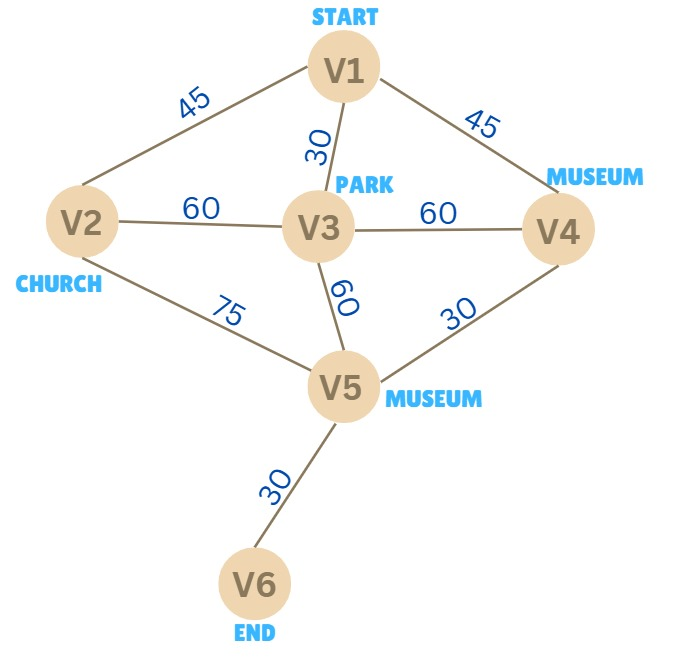
\includegraphics[width=0.5\textwidth]{image3.jpg}
% \end{figure}

% % \vspace{10cm}

% \begin{table}[ht]
% \centering
% \begin{tabular}{|c|c|c|c|}
% \hline
% POI & Category & Visit Time & Utility Score \\
% \hline
% \( v_1 \) & Start & 0 & 0  \\
% \( v_2 \) & Church & 90 & 20  \\
% \( v_3 \) & Park & 60 & 35 \\
% \( v_4 \) & Museum & 120 & 15 \\
% \( v_5 \) & Museum & 120 & 40 \\
% \( v_6 \) & End & 0 & 0 \\
% \hline
% \end{tabular}
% \caption{POI Details}
% \end{table}

% \subsection{Best Itinerary considering the category constraint}
% \textbf{Itinerary:}  
% \( V_1 \to V_2 \to V_5 \to V_6 \) \\

% \begin{itemize}
%     \item \textbf{Time Taken:}
%     \begin{itemize}
%     \item Travel \( V_1 \to V_2 \) = 45 min
%     \item Visit \( V_2 \) = 90 min
%     \item Travel \( V_2 \to V_5 \) = 75 min
%     \item Visit \(V_5\) = 120 min
%     \item Travel \(V_5 \to V_6 \) = 30 min
%     \end{itemize}
%     \item \textbf{Total Time: } 6 hours
%     \item \textbf{Utility Score: } 60
% \end{itemize}

% \begin{tcolorbox}[colback=gray!10,colframe=black,boxrule=0.5pt,left=2pt,right=2pt,top=2pt,bottom=2pt]
% \textbf{Note:} Although the utility score achieved by keeping the category constraint is 60, as shown in the next section, an even higher utility score can be achieved if the category constraint is removed.
% \end{tcolorbox}

% \subsection{Without considering the category constraint}
% \textbf{Best Itinerary:}  
% \( V_1 \to V_3 \to V_5 \to V_6 \) \\

% \begin{itemize}
% \item \textbf{Time Taken:}  
%     \begin{itemize}
%     \item Travel \( V_1 \to V_3 \) = 30 min 
%     \item Visit \( V_3 \) = 60 min  
%     \item Travel \( V_3 \to V_5 \) = 60 min
%     \item Visit \( V_5 \) = 120 min 
%     \item Travel \( V_5 \to V_6 \) = 30 min
%     \end{itemize}
% \item \textbf{Total time: }5 hours

% \item \textbf{Utility Score:}  
% \( 75 \) \\
% \end{itemize}

% \section{Dynamic Setting}
% \subsection{Overview}
% The $run\_optimizer$ function is responsible for dynamically optimizing a tourist’s travel itinerary using the Gurobi solver. It considers multiple constraints, including time, cost, and category-based constraints, ordering constraints, while maximizing the overall utility of the trip. This function enables real-time adjustments based on user interactions and previously visited points of interest (POIs).\\

% \noindent \textbf{Travel Time Calculation} \\
% The function calls Routes API of google maps in batch mode to obtain travel time matrices for two transportation modes: walking and taxi. It provides routes for driving and walking and calculates travel times and distances.

% \subsection{Objective Function}

% The objective is to \textbf{maximize the utility score} of the itinerary, which is the sum of the utility values of the selected POIs, while ensuring that already visited POIs are not reselected.

% \begin{align}
% \max \sum_{i \notin \text{visited\_pois}, i \neq \text{source\_poi}} \text{utility\_scores}[i] \cdot y[I] \label{25}
% \end{align}

% \subsection{Starting and Ending Point Constraint}
% \noindent
% This constraint ensures that exactly one outgoing edge is selected from the source node, which is dynamically determined as \texttt{source\_poi}, rather than being fixed. The selected edge should not go to any previously visited POI, and no incoming edge should be selected for \texttt{source\_poi}.  

% Similarly, for the ending node of the itinerary, denoted as $v_N$, exactly one incoming edge must be selected from an unvisited POI, and no outgoing edge should be chosen from $v_N$.  

% Mathematically, this is expressed as follows:
% \begin{align}
% \sum_{\substack{j \in \text{poi\_ids} \\ j \neq \text{source\_poi} \\ j \notin \text{visited\_pois}}} z_{\text{source\_poi}, j} &= 1 \label{26} \\  
% \sum_{\substack{i \in \text{poi\_ids} \\ i \neq \text{ending\_poi} \\ i \notin \text{visited\_pois}}} z_{i, \text{ending\_poi}} &= 1 \label{27} \\
% \sum_{\substack{i \in \text{poi\_ids} \\ i \neq \text{source\_poi} \\ i \notin \text{visited\_pois}}} z_{i, \text{source\_poi}} &= 0 \label{28} \\
% \sum_{\substack{j \in \text{poi\_ids} \\ j \neq \text{ending\_poi}}} z_{\text{ending\_poi}, j} &= 0 \label{29}
% \end{align}

% where $z_{i,j}$ is a binary variable that takes value $1$ if the path from node $v_i$ to $v_j$ is selected in the itinerary; and $0$ otherwise. Here, \texttt{source\_poi} represents the dynamically selected starting node, while $v_N$ denotes the fixed ending node of the itinerary. The total number of POIs is assumed to be $N$.  

% \subsection{No Self Loops}
% This constraint ensures that there is no edge from any vertex to itself.

% \begin{align}
% z[i, i] = 0 \quad \forall i \in V \label{30}
% \end{align}

% \subsection{Connectivity Constraint}

% \noindent
% This constraint ensures that:
% \begin{itemize}
%     \item Each Point of Interest (POI) can be \textbf{visited at most once}, preventing cycles or repeated visits to the same node.
%     \item All selected nodes are \textbf{connected in a single continuous path}.
% \end{itemize}

% In the dynamic approach, the connectivity constraint is applied to all POIs except the dynamically chosen starting node (\texttt{source\_poi}) and the fixed ending node $v_N$. Additionally, previously visited POIs are excluded from consideration. 

% Mathematically, for any intermediate POI $v_k \in V \setminus \{\texttt{source\_poi}, v_N\}$ that has not been visited in a prior itinerary ($k \notin \text{visited\_pois}$), exactly one incoming edge and one outgoing edge must be selected in the itinerary:

% \begin{align}
% \sum_{\substack{i \in \text{poi\_ids} \\ i \neq k \\ i \notin \text{visited\_pois} \\ k \notin \text{visited\_pois}}} z_{i,k} &= y[k], \quad \forall k \in V \setminus \{\texttt{source\_poi}, v_N\} \label{31} \\  
% \sum_{\substack{j \in \text{poi\_ids} \\ j \neq k \\ j \notin \text{visited\_pois} \\ k \notin \text{visited\_pois}}} z_{k,j} &= y[k], \quad \forall k \in V \setminus \{\texttt{source\_poi}, v_N\} \label{32}  
% \end{align}

% where $z_{i,j}$ is a binary variable that takes the value $1$ if the path from node $v_i$ to $v_j$ is selected in the itinerary, and $0$ otherwise. The variable $y[k]$ is an indicator variable ensuring that if POI $v_k$ is visited, it has exactly one incoming edge and one outgoing edge, maintaining connectivity.  

% \subsection{Logical Connection Between Variables \( y \) and \( z \)}

% \noindent  
% This constraint ensures that \( z_{i,j} = 1 \) only if both \( y_i = 1 \) and \( y_j = 1 \), while also excluding previously visited POIs.  

% Mathematically, this is expressed as:  

% \begin{align}
% z_{i,j} &\leq y_i, \quad \forall i, j \in V \setminus \text{visited\_pois}, \ i \neq j \label{33} \\
% z_{i,j} &\leq y_j, \quad \forall i, j \in V \setminus \text{visited\_pois}, \ i \neq j \label{34} \\
% y_i &\leq \sum_{\substack{j \in V \setminus \text{visited\_pois} \\ j \neq i}} z_{i,j}, \quad \forall i \in V \setminus \text{visited\_pois} \label{35}\\  
% y_j &\leq \sum_{\substack{i \in V \setminus \text{visited\_pois} \\ i \neq j}} z_{i,j}, \quad \forall j \in V \setminus \text{visited\_pois} \label{36} 
% \end{align}

% where \( V \setminus \text{visited\_pois} \) represents the set of POIs that have not been visited in a prior itinerary.  


% \subsection{Time Constraint Formulation}

% The total time spent traveling and visiting POIs in the further itinerary must not exceed the remaining time budget. This is formulated as:

% \begin{align}
% \sum_{\substack{i, j \in \text{poi\_ids}, \\ i \neq j, (i, j) \notin \text{visited\_edges}}} 
% \Big( t^{w}_{i,j} \cdot w_{i,j} + 
% t^{x}_{i,j} \cdot x_{i,j} \Big) + 
% \sum_{\substack{i \in \text{poi\_ids}, \\i \notin \{\text{starting\_poi}, \text{ending\_poi}\},\\ i \notin \text{visited\_pois}}} 
% \text{visit\_times}[i] \cdot y_i 
% \leq \text{remaining\_time\_budget} \label{37}
% \end{align}


% where:
% \begin{itemize}
%     \item $w_{i,j}$ and $x_{i,j}$ are binary decision variables indicating travel mode (walking or taxi) between POIs $i$ and $j$.
%     \item $\text{visited\_edges}$ represents already traversed edges and $\text{visited\_pois}$ represents already traversed pois that are excluded from consideration.
%     \item $y_i$ is a binary variable indicating whether POI $i$ is selected.
%     \item $\text{visit\_times}[i]$ denotes the visit duration for POI $i$.
% \end{itemize}

% \subsection{Cost Budget Constraint}

% The total cost, including travel costs and entrance fees of further itinerary, must not exceed the remaining cost budget. This is formulated as:

% \begin{align}
% \sum_{\substack{(i, j) \in \text{I},\\ (i, j) \notin \text{visited\_edges} }} 
%  \Big( t^{x}_{i,j} \cdot \text{taxi\_cost\_per\_min} \cdot x_{i,j} \Big)
% + \sum_{\substack{i \in \text{I} \\ i \notin \text{visited\_pois},\\ i \neq \text{source\_poi}}} 
% c(v_i)
% & \leq \text{remaining\_cost\_budget} \label{38}
% \end{align}

% where:
% \begin{itemize}
%     \item $x_{i,j}$ is a binary decision variable indicating whether a taxi is used between POIs $i$ and $j$.
%     \item $t^{x}_{i,j}$ provides the travel time by taxi between $i$ and $j$.
%     \item $\text{taxi\_cost\_per\_min}$ is the cost per minute for using a taxi.
%     \item $c(v_i)$ represents the entrance fee for POI $i$.
%     \item $\text{visited\_pois}$ are previously visited POIs that are excluded.
%     \item $\text{visited\_edges}$ are previously visited edges that are excluded.
%     \item $\text{remaining\_cost\_budget}$ is the dynamically updated budget.
% \end{itemize}

% \subsection{Category Constraint}
% \begin{itemize}
%     \item The number of POIs selected from each category is bounded by predefined lower and upper limits.
%     \item Let \( C \) denote the set of all categories.
%     \item For each category \( m \in C \), let \( V_m \subseteq V \) represent the set of POIs belonging to that category.
%     \item Let \( y_i \) be a binary variable where \( y_i = 1 \) if POI \( v_i \) is included in the itinerary, and \( y_i = 0 \) otherwise.
%     \item Let \( lb_m \) and \( ub_m \) denote the lower and upper bounds, respectively, on the number of POIs to be selected from category \( m \).

%     \begin{align}
%     lb_m \leq \sum_{\substack{i \in V_m}} y_i \leq ub_m, \quad \forall m \in C \label{39}
% \end{align}


%     \item The value of \( lb_k \) for any mandatory category \(k \in m\) will be 1.
% \end{itemize}

% Rest all the constraints are the same as those in the static approach

% \subsection{Fractional Visit to POI}

% \textbf{What is Fractional Utility?} \\
% In our trip itinerary planning system, each Point of Interest (POI) is associated with a utility value representing how beneficial or enjoyable it is for a tourist to visit that location. The optimization model aims to maximize the total utility while adhering to constraints such as total travel time and budget.

% However, due to limited time and resources, it might not always be feasible to fully visit every POI. To address this, we introduce the concept of \textit{fractional utility}.

% \textbf{Why Use It?}
% \begin{itemize}
%     \item Makes the itinerary more flexible, especially when time is tight.
%     \item Encourages optimal use of time, distributing it across several POIs instead of visiting fewer places completely.
%     \item Helps avoid hard binary decisions that might lead to lower overall utility.
% \end{itemize}

% \subsection{Modeling Fractional Utility and Slab Constraints}

% In order to allow partial visits to Points of Interest (POIs), we introduce a continuous decision variable \( \text{ppoi}_i \in [0, 1] \), representing the fraction of time spent at POI \( i \), and consequently, the fraction of utility gained.

% The following constraints ensure a consistent and logical relationship between \( \text{ppoi}_i \) and \( y_i \):

% \begin{align}
% \text{ppoi}_i &\geq 0.5 \cdot y_i && \text{(If POI is selected, it must be visited at least 50\%)} \\
% \text{ppoi}_i &\leq (0.5 - \epsilon) + y_i && \text{(If } \text{ppoi}_i \geq 0.5 \text{, then } y_i = 1) \\
% \text{ppoi}_i &\leq y_i && \text{(If } y_i = 0 \text{, then } \text{ppoi}_i = 0) \\
% \text{ppoi}_i &\geq (0.5 - \epsilon) - (1 - y_i) && \text{(If } \text{ppoi}_i < 0.5 \text{, then } y_i = 0)
% \end{align}

% To control how utility is computed based on time spent, we define \textbf{slabs} using binary variables \( s1_i, s2_i, s3_i \in \{0,1\} \), where:
% \begin{itemize}
%     \item \( s1_i = 1 \): POI is visited between 50\% and 70\%, 60\% utility will be awarded
%     \item \( s2_i = 1 \): POI is visited between 70\% and 90\%, 80\% utility will be awarded
%     \item \( s3_i = 1 \): POI is visited more than 90\%, 100\% utility will be awarded
% \end{itemize}

% Each POI can belong to at most one slab:
% \begin{equation}
% s1_i + s2_i + s3_i \leq 1
% \end{equation}

% We then connect the fractional visit time \( \text{ppoi}_i \) to the selected slab:
% \begin{align}
% \text{ppoi}_i &\geq 0.5 \cdot s1_i + 0.7 \cdot s2_i + 0.9 \cdot s3_i \\
% \text{ppoi}_i &\leq (0.7 - \epsilon) \cdot s1_i + (0.9 - \epsilon) \cdot s2_i + s3_i
% \end{align}

% Finally, we define an auxiliary variable \( \text{effective\_utility}_i \) that captures the utility earned from POI \( i \) based on the slab:
% \begin{equation}
% \text{effective\_utility}_i = \text{utility\_score}_i \cdot (0.6 \cdot s1_i + 0.8 \cdot s2_i + 1.0 \cdot s3_i)
% \end{equation}

% This ensures that utility is gained only in \textbf{discrete slabs} based on the extent of time spent at each POI, rather than being a continuous linear function, making the model more realistic in terms of tourist experience.

% \subsection{Updated Constraints and Objective Function}

% Due to the integration of fractional utility slabs and partial POI visits, several constraints and the objective function in our optimization model have been revised. These updates ensure that the model accurately reflects time-budgeted, partial POI experiences while maintaining feasibility in terms of travel and time windows.

% \subsubsection*{Objective Function}

% The goal is now to maximize the total effective utility based on the selected slabs for each POI:
% \begin{align}
% \max \sum_{i \notin \text{visited\_pois}, i \neq \text{source\_poi}} \text{effective\_utility\_scores}[i] \label{25}
% \end{align}
% Here, effective utility is computed using the slab-based utility mapping.

% \subsubsection*{Time Constraint}

% The total time spent must not exceed the remaining time budget. The time consists of three parts:
% \begin{itemize}
%     \item Time spent walking
%     \item Time spent using taxis
%     \item Time spent at POIs based on fractional visit time \( \text{ppoi}_i \)
% \end{itemize}
% \begin{align}
% \sum_{\substack{i, j \in \text{poi\_ids}, \\ i \neq j, (i, j) \notin \text{visited\_edges}}} 
% \Big( t^{w}_{i,j} \cdot w_{i,j} + 
% t^{x}_{i,j} \cdot x_{i,j} \Big) + 
% \sum_{\substack{i \in \text{poi\_ids}, \\i \notin \{\text{starting\_poi}, \text{ending\_poi}\},\\ i \notin \text{visited\_pois}}} 
% \text{visit\_times}[i] \cdot ppoi_i 
% \leq \text{remaining\_time\_budget} \label{37}
% \end{align}

% \subsubsection*{Arrival Time Calculation}

% To ensure the correct ordering and timing of visits, the arrival time at a POI \( i \) must be greater than or equal to the sum of:
% \begin{itemize}
%     \item Arrival time at POI \( j \)
%     \item Time spent at POI \( j \) (adjusted by fraction \(\text{ppoi}_j\))
%     \item Travel time from POI \( j \) to \( i \)
% \end{itemize}
% \begin{equation}
% \text{arrival\_time}_i \geq 
% \left( \text{arrival\_time}_j + \text{visit\_time}_j \cdot \text{ppoi}_j +
% \text{travel\_time}_{ji} \right) \cdot z_{ji}
% \end{equation}
% Where \( z_{ji} \) is a binary variable indicating a transition from POI \( j \) to POI \( i \).

% \subsubsection*{Opening and Closing Time Constraints}

% To respect the visiting hours of each POI, we impose the following constraints:
% \begin{align}
% \text{arrival\_time}_i &\geq \text{opening\_time}_i \\
% \text{arrival\_time}_i + \text{visit\_time}_i \cdot \text{ppoi}_i &\leq \text{closing\_time}_i
% \end{align}
% These ensure that each POI is visited only within its available time window, considering partial visits.



% \vspace{1em}


% \section{Related Work}

% Taylor et al. (2018) introduced the \textit{TourMustSee problem}, focusing on integrating must-visit POIs into itineraries using their \textit{LP+M algorithm}. Their model ensures must-see POIs are included while optimizing tour duration and POI popularity, using real-life data from Flickr~\cite{taylor2018tour}.

% The \textit{Tourist Trip Design Problem (TTDP)}, an extension of the Orienteering Problem, has been widely studied to help tourists plan optimal itineraries under practical constraints. Vu et al. (2022) proposed a \textit{branch-and-check} approach for TTDP with complex constraints such as budget, time windows, and mandatory visits, ensuring feasible solutions through a combination of master and sub-problems~\cite{vu2022branch}.

% Taylor et al. (2018) introduced the \textit{TourMustSee problem}, focusing on integrating must-visit POIs into itineraries using their \textit{LP+M algorithm}. Their model ensures must-see POIs are included while optimizing tour duration and POI popularity, using real-life data from Flickr~\cite{taylor2018tour}.

% While these works address various constraints, they mainly rely on single-mode transportation models like walking or fixed travel times. In contrast, our work models the problem using a \textit{multimodal graph} with walking and taxi modes, adding a \textit{user-defined walking time threshold} to limit continuous walking duration. Additionally, we incorporate the operating days of POIs (i.e., whether a POI is open or closed on a specific day), a factor that has not been considered in previous studies. This makes our approach more practical and comprehensive for real-world itinerary planning.

\bibliographystyle{ACM-Reference-Format}
\bibliography{references}

\end{document}
